\documentclass[12pt,a4paper,oneside]{book}

% Load preamble (fonts, packages, styling)
% ==============================================================================
% PREAMBLE: The Chimera Project - LaTeX Package Configuration and Styling
% ==============================================================================

% ==============================================================================
% FONTS AND TYPESETTING
% ==============================================================================
\usepackage{fontspec}

% Set main fonts (with fallbacks)
\setmainfont{Latin Modern Roman}[
  Ligatures=TeX,
  Numbers=OldStyle
]

\setsansfont{Latin Modern Sans}[
  Ligatures=TeX,
  Scale=MatchLowercase
]

\setmonofont{Latin Modern Mono}[
  Scale=MatchLowercase
]

% Define custom font commands for title page
\newfontfamily\trajantitle{Latin Modern Roman}[
  Ligatures=TeX,
  Scale=1.2
]

% ==============================================================================
% CORE PACKAGES
% ==============================================================================

% --- Page Layout ---
\usepackage[
  paperwidth=7in,
  paperheight=10in,
  top=0.75in,
  bottom=0.75in,
  inner=0.75in,
  outer=0.5in,
  includehead,
  includefoot
]{geometry}

% --- Mathematics ---
\usepackage{amsmath}
\usepackage{amssymb}
\usepackage{amsthm}
\usepackage{mathtools}

% --- Graphics and Color ---
\usepackage{graphicx}
\usepackage{xcolor}
\usepackage{tikz}
\usetikzlibrary{calc,patterns,decorations.pathmorphing,decorations.markings}

% Define custom colors
\definecolor{NavyBlue}{RGB}{0,47,108}
\definecolor{BoxBg}{RGB}{245,245,250}

% --- PDF Handling ---
\usepackage{pdfpages}

% --- Hyperlinks ---
\usepackage{hyperref}
\hypersetup{
  colorlinks=true,
  linkcolor=NavyBlue,
  filecolor=NavyBlue,
  urlcolor=NavyBlue,
  citecolor=NavyBlue,
  bookmarks=true,
  bookmarksopen=true,
  pdfstartview=FitH
}

% --- Bibliography ---
\usepackage[
  backend=biber,
  style=numeric,
  sorting=none,
  maxbibnames=99
]{biblatex}
\addbibresource{bibliography.bib}

% --- Index ---
\usepackage{makeidx}
\makeindex

% ==============================================================================
% CUSTOM ENVIRONMENTS
% ==============================================================================

% --- Colored Boxes (tcolorbox) ---
\usepackage{tcolorbox}
\tcbuselibrary{skins,breakable}

% Base box style
\tcbset{
  base/.style={
    enhanced,
    breakable,
    colback=white,
    colframe=NavyBlue,
    boxrule=1pt,
    sharp corners,
    left=8pt,
    right=8pt,
    top=6pt,
    bottom=6pt,
    toptitle=3pt,
    bottomtitle=3pt
  }
}

% Non-technical callout (light blue background)
\newtcolorbox{nontechnical}{
  base,
  colback=BoxBg,
  colframe=NavyBlue,
  title={\textbf{Non-Technical Summary}},
  fonttitle=\sffamily\bfseries
}

% Key concept box
\newtcolorbox{keyconcept}{
  base,
  colback=yellow!5,
  colframe=orange!70!black,
  title={\textbf{Key Concept}},
  fonttitle=\sffamily\bfseries
}

% Important box
\newtcolorbox{importantbox}{
  base,
  colback=red!5,
  colframe=red!70!black,
  title={\textbf{Important}},
  fonttitle=\sffamily\bfseries
}

% Warning box
\newtcolorbox{warningbox}{
  base,
  colback=orange!5,
  colframe=orange!80!black,
  title={\textbf{Warning}},
  fonttitle=\sffamily\bfseries
}

% Generic callout box with optional title
\newtcolorbox{calloutbox}[1][]{
  base,
  colback=BoxBg,
  colframe=NavyBlue,
  title={#1},
  fonttitle=\sffamily\bfseries
}

% ==============================================================================
% TABLES AND LISTS
% ==============================================================================

% --- Tables ---
\usepackage{array}
\usepackage{longtable}
\usepackage{booktabs}
\usepackage{tabularx}
\usepackage{calc}

% Define \real for pandoc-generated table column widths
\providecommand{\real}[1]{#1}

% --- Lists ---
\usepackage{enumitem}
\setlist{noitemsep, topsep=5pt}

% Pandoc compatibility - define \tightlist for compact lists
\providecommand{\tightlist}{%
  \setlength{\itemsep}{0pt}\setlength{\parskip}{0pt}}

% ==============================================================================
% CHAPTER AND SECTION STYLING
% ==============================================================================
\usepackage{titlesec}

% Chapter formatting
\titleformat{\chapter}[display]
  {\sffamily\bfseries\Large}
  {\chaptertitlename\ \thechapter}{12pt}{\fontsize{24}{28}\selectfont}
\titlespacing*{\chapter}{0pt}{-30pt}{20pt}

% Section formatting
\titleformat{\section}
  {\sffamily\bfseries\large}
  {\thesection}{1em}{}

% Subsection formatting
\titleformat{\subsection}
  {\sffamily\bfseries\normalsize}
  {\thesubsection}{1em}{}

% Subsubsection formatting
\titleformat{\subsubsection}
  {\sffamily\bfseries\normalsize}
  {\thesubsubsection}{1em}{}

% ==============================================================================
% TABLE OF CONTENTS CONFIGURATION
% ==============================================================================

\setcounter{tocdepth}{2}  % Show chapters, sections, subsections
\setcounter{secnumdepth}{3}  % Number up to subsubsections

% TOC formatting
\usepackage{tocloft}

% Part entries in TOC
% Using \sffamily for sans-serif
\renewcommand{\cftpartfont}{\sffamily\bfseries\Large}
\renewcommand{\cftpartpagefont}{\sffamily\bfseries\Large}
\setlength{\cftbeforepartskip}{2em}

% Chapter entries in TOC
\renewcommand{\cftchapfont}{\sffamily\bfseries}
\renewcommand{\cftchappagefont}{\sffamily\bfseries}
\setlength{\cftbeforechapskip}{0.8em}
\renewcommand{\cftchapleader}{\cftdotfill{\cftdotsep}}

% Section entries in TOC
\renewcommand{\cftsecfont}{\sffamily}
\renewcommand{\cftsecpagefont}{\sffamily}
\setlength{\cftbeforesecskip}{0.4em}
\setlength{\cftsecindent}{1.5em}

% Subsection entries in TOC
% Using normal font (serif) for subsections to provide visual hierarchy
\renewcommand{\cftsubsecfont}{\normalfont}
\renewcommand{\cftsubsecpagefont}{\normalfont}
\setlength{\cftbeforesubsecskip}{0.2em}
\setlength{\cftsubsecindent}{3em}

% ==============================================================================
% CUSTOM COMMANDS
% ==============================================================================

% Key term highlighting
\newcommand{\keyterm}[1]{\textbf{\textcolor{NavyBlue}{#1}}}

% Paragraph heading
\newcommand{\parhead}[1]{\paragraph{#1}}

% Logged input (for debugging chapter loading)
\newcommand{\loggedinput}[1]{%
  \typeout{LOADING CHAPTER: #1}%
  \input{#1}%
  \typeout{CHAPTER #1 COMPLETE}%
}

% ==============================================================================
% MISCELLANEOUS SETTINGS
% ==============================================================================

% Prevent overfull hbox warnings for slight overruns
\tolerance=1000
\hbadness=1000

% Allow more flexible float placement
\renewcommand{\topfraction}{0.85}
\renewcommand{\bottomfraction}{0.85}
\renewcommand{\textfraction}{0.1}
\renewcommand{\floatpagefraction}{0.75}

% ==============================================================================
% END OF PREAMBLE
% ==============================================================================


% Book metadata
\title{Chimera: Signals Processing, Past, Present \& Future}
\author{Edited by Rowan Jones}
\date{First Edition, \today}

\begin{document}

% Front Matter
\frontmatter

% Cover page with cover art
\begin{titlepage}
\centering
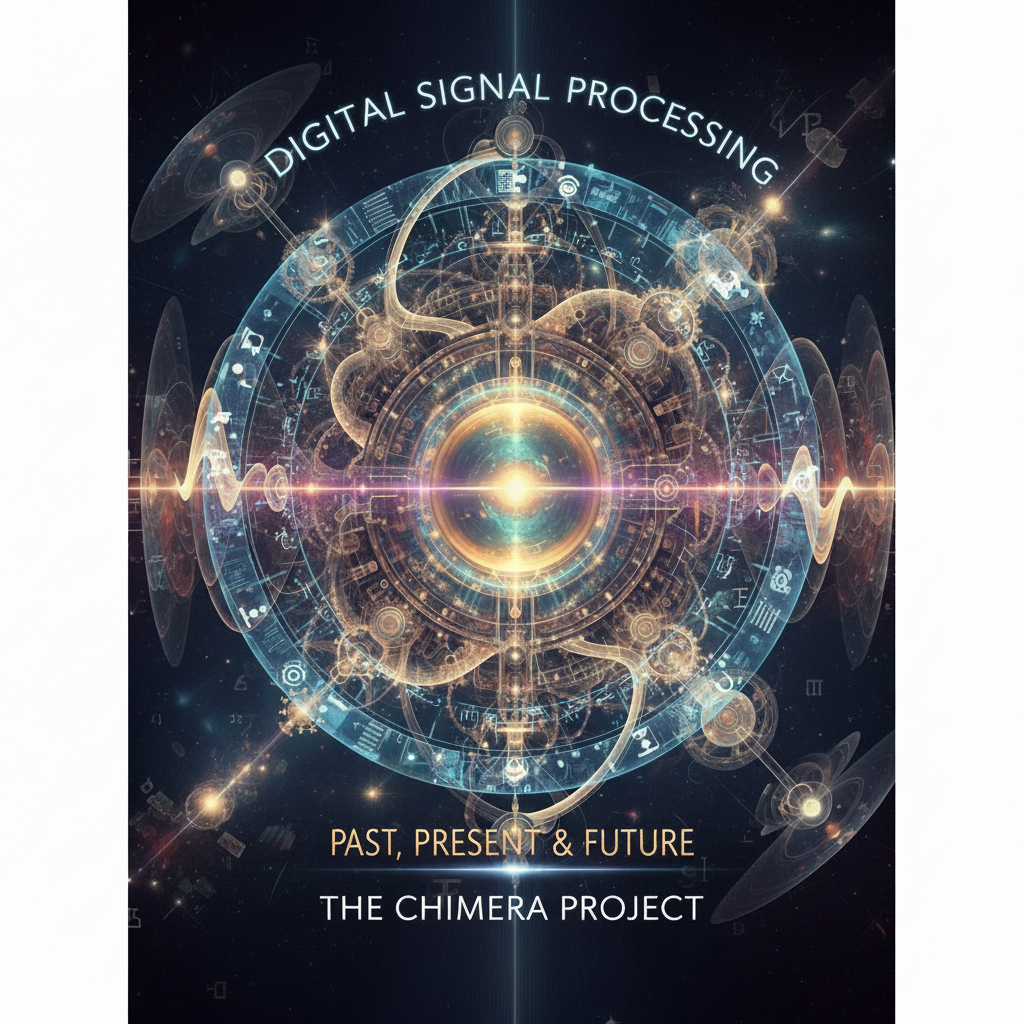
\includegraphics[width=\textwidth,height=\textheight,keepaspectratio]{graphics/cover_art.png}
\end{titlepage}

% Title page
\begin{titlepage}
    \centering
    \vspace*{2cm}
    
    {\Huge\bfseries\color{NavyBlue} Chimera: Signals Processing, Past, Present \& Future\par}
    \vspace{1cm}
    {\Large\itshape Rowan Jones\par}
    \vspace{0.2cm}
    {\small\href{mailto:rowan@impermanent.io}{rowan@impermanent.io}\par}
    {\small\url{www.impermanent.io}\par}
    \vspace{0.5cm}
    {\large \today\par}
    
    \vspace{2cm}
    
    {\large\itshape
    A comprehensive guide to digital signal processing,\\
    wireless communications, and paradigm-challenging technologies.\par}
    
    \vfill
    
\end{titlepage}


% Copyright/License page
\newpage
\thispagestyle{empty}
\vspace*{\fill}
\begin{center}

{\Large\bfseries Chimera: Signals Processing, Past, Present \& Future}

\vspace{1cm}

{\large First Edition}

\vspace{0.5cm}

{\large Edited by Rowan Jones}

\vspace{1cm}

Published by The Chimera Project\\
\href{mailto:chimera@impermanent.io}{chimera@impermanent.io}\\
\url{www.impermanent.io}

\vspace{1cm}


\includegraphics[width=3cm]{graphics/cc-zero.png}

\vspace{0.5cm}

{\large CC0 1.0 Universal (Public Domain)}

\vspace{0.5cm}

To the extent possible under law, The Chimera Project has waived all copyright and related or neighboring rights to this work. This work is published from: Australia.

\vspace{1cm}

{\small Typeset in \LaTeX{} with Libertinus fonts and Cabin headings.}

\vspace{0.5cm}

{\small Cover art: \textit{[Cover Art Credit]}}

\end{center}
\vspace*{\fill}
\newpage

% Dedication
\newpage
\thispagestyle{empty}

\vspace*{\fill}

\begin{center}
\begin{minipage}{0.7\textwidth}
\centering

\textit{In memory of Alan Turing, a brilliant mind persecuted for who he was.}

\vspace{1.5cm}

\textit{And to the 27 Unnamed Women and the countless others who have endured untold suffering at the hands of a project that bears his name but has betrayed his humane spirit.}

\vspace{3cm}

To those I have harmed in this process, I am deeply sorry.

\vspace{2.5cm}

For Saba, my parents, and all who have stood with me through this ordeal—thank you for everything.

\vspace{3.5cm}

\textit{May the words in this book bring some measure of peace to a troubled world.}

\vspace{1.5cm}

\textit{May you be happy, may you be safe, may you be well.}

\vspace{3cm}

\textit{For all that has been done, and all we have yet to do.}

\vspace{3.5cm}

{\large\textbf{\textit{Be Not Afraid.}}}

\end{minipage}
\end{center}

\vspace*{\fill}
\newpage

% Foreword
\newpage
\thispagestyle{empty}

\vspace*{3cm}

\begin{center}
{\Large\textsc{Foreword}}
\end{center}

\vspace{2cm}

\begin{center}

There will come a time in your life when you will ask yourself a series of questions.

\vspace{1.2cm}
\textit{Am I happy with who I am?}\\
\textit{Am I happy with the people around me?}\\
\textit{Am I happy with what I'm doing?}\\
\textit{Am I happy with the way my life is going?}\\
\textit{Do I have a life or am I just living?}
\vspace{1.2cm}

\textbf{Do not let these questions strain or trouble you---just point yourself in the direction of your dreams, find your strength in the sound, and \emph{make your transition}}.

\vspace{2cm}

Do not spend too much time thinking and not enough doing.

\vspace{1.2cm}
\textit{Did I try the hardest at any of my dreams?}\\
\textit{Did I purposely let others discourage me when I knew I could?}\\
\textit{Will I die never knowing what I could have been or could have done?}
\vspace{1.2cm}

\textbf{Do not let these doubts restrain or trouble you---just point yourself in the direction of your dreams. Find your strength in the sound and \emph{make your transition}}.

\vspace{2.5cm}

There will be people who say you can't---\textbf{you will.}\\[0.8cm]
There will be people who say you don't mix this with that,\\
and you will say ``\textbf{watch me}.''\\[0.8cm]
There will be people who will say play it safe, that's too risky---\\
\textbf{you will take that chance and have no fear.}\\[1.5cm]

\textbf{You won't let these questions restrain or trouble you.}\\
\textbf{You will point yourself in the direction of your dreams.}\\
\textbf{You will find the strength in the sound and \emph{make your transition}.}

\vspace{2.5cm}

For those who know it's time to leave the house and go back to the field:\\[1cm]
{\Large\textbf{Find your strength in the sound and \emph{make your transition}.}}

\end{center}

\vspace{2cm}

\begin{flushright}
\textit{--- Underground Resistance, ``Transition''}
\end{flushright}

\vspace*{\fill}

\newpage


% Table of Contents
\tableofcontents
\newpage

% Introduction
\chapter*{Introduction}
\addcontentsline{toc}{chapter}{Introduction}

\begin{nontechnical}
This book is intended for a wide audience, from students of signal processing to seasoned engineers and researchers. While the foundational chapters provide a solid grounding in established theory, the later sections venture into more speculative and paradigm-challenging territory. These advanced topics are presented not as established fact, but as an invitation to explore the boundaries of our current understanding. They are the result of extensive research and experimentation, and are intended to spark curiosity and debate. We encourage readers to approach this material with an open and critical mind, to question assumptions, and to join us in the exciting quest for new knowledge.
\end{nontechnical}

\vspace{1cm}

The journey you are about to embark on is one of discovery. It begins with the well-trodden paths of digital signal processing (DSP) and wireless communications, but it does not end there. The Chimera project was born from a desire to not only understand the world of signals, but to question its very foundations.

In the following chapters, you will find a comprehensive exploration of the principles that govern our modern connected world. But you will also find something more: a challenge. A challenge to the conventional models, a questioning of long-held assumptions, and a presentation of new ideas that may, at first, seem outlandish.

This is by design. True innovation does not come from accepting the status quo, but from daring to ask "what if?". The advanced concepts presented here, particularly those related to biophysical communication and hyper-rotational physics, are the product of that question. They are presented here not as dogma, but as a starting point for a new conversation.

Whether you are a student seeking to learn, a hobbyist looking to experiment, or a researcher searching for the next frontier, we hope this work provides you with both the tools to build and the inspiration to dream.

Welcome to Chimera.


% Main Content
\mainmatter

% Include all chapters (alphabetically)
% Wave 1: Exemplar (complete)
\chapter{Binary Phase-Shift Keying (BPSK)}
\label{ch:bpsk}

\begin{nontechnical}
\textbf{BPSK is like Morse code with a twist}---instead of turning a signal on and off, you flip the wave upside-down to send 1s and 0s.

\textbf{Simple idea:}
\begin{itemize}
\item Bit 0 = wave pointing ``up'' $\uparrow$
\item Bit 1 = wave pointing ``down'' $\downarrow$ (flipped $180°$)
\end{itemize}

\textbf{Real use:} GPS satellites use BPSK. Your phone detects whether the signal is normal or flipped.

\textbf{Why flip instead of on/off?} More reliable in noise, works with constant power, less interference. Trade-off: Simple but slow (1 bit per symbol).
\end{nontechnical}

\section{Overview}

\textbf{Binary Phase-Shift Keying (BPSK)} is the simplest form of phase modulation, where binary data is encoded by shifting the carrier phase between two states: $0°$ and $180°$.

\begin{keyconcept}
BPSK provides \textbf{3~dB better performance} than On-Off Keying (OOK) at the same signal-to-noise ratio, making it the optimal choice for power-limited channels such as satellite and deep-space communications.
\end{keyconcept}

BPSK forms the foundation for higher-order phase shift keying schemes including QPSK (4 phases), 8PSK (8 phases), and beyond.

\section{Mathematical Description}

\subsection{Time-Domain Signal}

The BPSK waveform is expressed as:
\begin{equation}
s(t) = A \cos(2\pi f_c t + \phi_n)
\end{equation}
where:
\begin{itemize}
\item $A$ = carrier amplitude
\item $f_c$ = carrier frequency (Hz)
\item $\phi_n \in \{0°, 180°\}$ = phase for bit $n$
\end{itemize}

\textbf{Phase encoding:}
\begin{equation}
\phi_n = \begin{cases}
0° & \text{if bit = 0} \\
180° & \text{if bit = 1}
\end{cases}
\end{equation}

\textbf{Alternative representation} using the cosine identity $\cos(\theta + 180°) = -\cos(\theta)$:
\begin{equation}
s(t) = A \cdot d_n \cdot \cos(2\pi f_c t)
\end{equation}
where $d_n \in \{+1, -1\}$ is the bipolar data symbol:
\begin{itemize}
\item Bit 0 $\rightarrow$ $d_n = +1$ $\rightarrow$ $0°$ phase
\item Bit 1 $\rightarrow$ $d_n = -1$ $\rightarrow$ $180°$ phase (inverted carrier)
\end{itemize}

\begin{calloutbox}{Physical Interpretation}
BPSK is effectively \textbf{amplitude modulation with bipolar data}. The carrier polarity flips between positive and negative, which is equivalent to a $180°$ phase shift. This representation simplifies both mathematical analysis and hardware implementation.
\end{calloutbox}

\section{IQ Representation}

The baseband complex representation of BPSK is:
\begin{equation}
s(t) = \mathrm{Re}\{A \cdot d_n \cdot e^{j2\pi f_c t}\}
\end{equation}

\textbf{IQ components:}
\begin{itemize}
\item \textbf{I (In-phase):} $I_n = A \cdot d_n$ (either $+A$ or $-A$)
\item \textbf{Q (Quadrature):} $Q_n = 0$ (BPSK uses only the I axis)
\end{itemize}

\subsection{Constellation Diagram}

The BPSK constellation consists of two points on the real axis separated by maximum distance $d = 2A$:

\begin{center}
\begin{tikzpicture}[scale=1.5]
% Axes
\draw[->] (-3,0) -- (3,0) node[right] {\sffamily\small $I$ (Real)};
\draw[->] (0,-2) -- (0,2) node[above] {\sffamily\small $Q$ (Imaginary)};

% Grid
\draw[very thin,gray!30] (-2.5,-1.5) grid[step=0.5] (2.5,1.5);

% Constellation points
\fill[black] (-2,0) circle (3pt);
\fill[black] (2,0) circle (3pt);

% Labels
\node[below=8pt,align=center] at (-2,0) {\sffamily\small Bit 1\\$(-A, 0)$\\$180°$};
\node[below=8pt,align=center] at (2,0) {\sffamily\small Bit 0\\$(+A, 0)$\\$0°$};

% Distance annotation
\draw[<->,thick] (-2,0.8) -- (2,0.8) node[midway,above] {\sffamily\small $d = 2A$};
\end{tikzpicture}
\end{center}

This maximum Euclidean separation between symbols provides optimal noise immunity for binary modulation schemes.

\section{Modulation and Demodulation}

\subsection{Transmitter (Modulator)}

The BPSK modulator consists of three stages:

\begin{center}
\begin{tikzpicture}[
  block/.style={rectangle, draw, minimum width=2.2cm, minimum height=1cm, font=\sffamily\small},
  node distance=2.2cm,
  font=\small
]
\node (input) {\sffamily Binary\\$\{0, 1\}$};
\node[block, right of=input, node distance=2.8cm] (nrz) {NRZ\\Encoder};
\node[block, right of=nrz, node distance=3.2cm] (mult) {Mixer\\$\times$};
\node[block, right of=mult, node distance=3cm] (filter) {Bandpass\\Filter};
\node[right of=filter, node distance=2.8cm] (output) {\sffamily BPSK\\Output};

\node[below of=mult, node distance=1.5cm, font=\small] (carrier) {$\cos(2\pi f_c t)$};

\draw[->,thick] (input) -- (nrz);
\draw[->,thick] (nrz) -- node[above,font=\scriptsize] {$d_n$} (mult);
\draw[->,thick] (carrier) -- (mult);
\draw[->,thick] (mult) -- (filter);
\draw[->,thick] (filter) -- (output);
\end{tikzpicture}
\end{center}

\textbf{Process:}
\begin{enumerate}
\item \textbf{NRZ encoding:} Map bits to bipolar symbols
  \begin{itemize}
  \item Bit 0 $\rightarrow$ $d_n = +1$
  \item Bit 1 $\rightarrow$ $d_n = -1$
  \end{itemize}
\item \textbf{Multiply by carrier:} $s(t) = A \cdot d_n \cdot \cos(2\pi f_c t)$
\item \textbf{Pulse shaping:} Apply raised-cosine filter to:
  \begin{itemize}
  \item Limit occupied bandwidth
  \item Prevent intersymbol interference (ISI)
  \item Meet spectral mask requirements
  \end{itemize}
\end{enumerate}

\subsection{Receiver (Coherent Detector)}

\begin{center}
\begin{tikzpicture}[
  block/.style={rectangle, draw, minimum width=2cm, minimum height=1cm, font=\sffamily\small},
  node distance=2cm,
  font=\small
]
\node (input) {\sffamily RX\\Signal};
\node[block, right of=input, node distance=2.5cm] (mult) {Mixer\\$\times$};
\node[block, right of=mult, node distance=2.8cm] (lpf) {Lowpass\\Filter};
\node[block, right of=lpf, node distance=2.8cm] (sample) {Sample\\$@T_s$};
\node[block, right of=sample, node distance=2.8cm] (thresh) {Threshold\\$>0?$};
\node[right of=thresh, node distance=2.8cm] (output) {\sffamily Data\\$\{0,1\}$};

\node[below of=mult, node distance=1.5cm, font=\scriptsize, align=center] (lo) {$2\cos(2\pi f_c t + \phi)$\\Local Oscillator};

\draw[->,thick] (input) -- (mult);
\draw[->,thick] (lo) -- (mult);
\draw[->,thick] (mult) -- (lpf);
\draw[->,thick] (lpf) -- (sample);
\draw[->,thick] (sample) -- (thresh);
\draw[->,thick] (thresh) -- (output);
\end{tikzpicture}
\end{center}

\begin{warningbox}
\textbf{Phase synchronization is critical.} The local oscillator must be exactly in phase with the transmitter carrier. A phase offset $\phi_e$ reduces detected signal by $\cos(\phi_e)$. At $\phi_e = 90°$, complete signal loss occurs.
\end{warningbox}

\textbf{Detection process:}

\begin{enumerate}
\item \textbf{Multiply by local carrier} (frequency $f_c$, phase $\phi = 0$):
\begin{equation}
r(t) = s(t) \cdot 2\cos(2\pi f_c t) = 2A d_n \cos^2(2\pi f_c t)
\end{equation}

\item \textbf{Apply trigonometric identity} $\cos^2(x) = \frac{1}{2}[1 + \cos(2x)]$:
\begin{equation}
r(t) = A d_n [1 + \cos(4\pi f_c t)]
\end{equation}

\item \textbf{Lowpass filter} removes $2f_c$ component, leaving baseband:
\begin{equation}
y(t) = A d_n
\end{equation}

\item \textbf{Sample at bit period} $T_b$: $y_n = A d_n + n(t)$ where $n(t)$ is AWGN

\item \textbf{Threshold decision:}
\begin{equation}
\hat{d}_n = \begin{cases}
+1 & \text{if } y_n > 0 \quad \text{(decode as bit 0)} \\
-1 & \text{if } y_n < 0 \quad \text{(decode as bit 1)}
\end{cases}
\end{equation}
\end{enumerate}

\section{Carrier Recovery}

The receiver must generate a local oscillator \textbf{exactly in phase} with the transmitter carrier. This is the primary challenge in coherent BPSK detection.

\subsection{Problem: Phase Ambiguity}

A phase offset $\phi_e$ between transmitter and receiver carriers causes:
\begin{equation}
y(t) = A d_n \cos(\phi_e) + n(t)
\end{equation}

\textbf{Effects:}
\begin{itemize}
\item $\phi_e = 0°$: Full signal strength (optimal)
\item $\phi_e = 45°$: Signal reduced by 3~dB
\item $\phi_e = 90°$: Complete signal loss
\item $\phi_e = 180°$: Inverted data (all bits flipped)
\end{itemize}

\subsection{Carrier Recovery Techniques}

\subsubsection{1. Pilot Tone}
\begin{itemize}
\item[\checkmark] Simple implementation
\item[\checkmark] Accurate phase reference
\item[\texttimes] Wastes power (typically 10--20\% of total)
\item[\texttimes] Reduces data throughput
\end{itemize}

\subsubsection{2. Costas Loop}
PLL-based carrier recovery using I/Q demodulation:
\begin{itemize}
\item[\checkmark] No pilot tone required
\item[\checkmark] Optimal for BPSK and QPSK
\item[\texttimes] Complex analog circuitry
\item[\texttimes] Acquisition time required
\end{itemize}

\subsubsection{3. Squaring Loop}
Exploits $d_n^2 = 1$ to remove data modulation:
\begin{equation}
[d_n \cos(2\pi f_c t)]^2 = \frac{1}{2}[1 + \cos(4\pi f_c t)]
\end{equation}
PLL locks to $2f_c$, then divides by 2 to recover $f_c$.
\begin{itemize}
\item[\checkmark] Completely removes data modulation
\item[\checkmark] Robust in low SNR
\item[\texttimes] $180°$ phase ambiguity (requires differential encoding)
\end{itemize}

\subsection{Differential BPSK (DBPSK)}

\textbf{Principle:} Encode data in \textbf{phase transitions}, not absolute phase.

\textbf{Encoding rule:}
\begin{equation}
\phi_n = \phi_{n-1} + \Delta\phi_n \quad\text{where}\quad \Delta\phi_n = \begin{cases}
0° & \text{if bit = 0} \\
180° & \text{if bit = 1}
\end{cases}
\end{equation}

\textbf{Decoding:} Compare consecutive symbols:
\begin{equation}
\hat{b}_n = \begin{cases}
0 & \text{if } \mathrm{sgn}(y_n) = \mathrm{sgn}(y_{n-1}) \\
1 & \text{if } \mathrm{sgn}(y_n) \neq \mathrm{sgn}(y_{n-1})
\end{cases}
\end{equation}

\textbf{Trade-off:}
\begin{itemize}
\item[\checkmark] No carrier recovery needed
\item[\checkmark] Simpler receiver
\item[\texttimes] Approximately 3~dB performance penalty
\item[\texttimes] Error propagation (single error affects two bits)
\end{itemize}

\section{Bit Error Rate (BER) Performance}

\subsection{Coherent BPSK in AWGN Channel}

For ideal coherent detection with perfect synchronization:
\begin{equation}
\mathrm{BER} = Q\left(\sqrt{\frac{2E_b}{N_0}}\right) = \frac{1}{2}\mathrm{erfc}\left(\sqrt{\frac{E_b}{N_0}}\right)
\end{equation}
where:
\begin{itemize}
\item $E_b = \frac{A^2 T_b}{2}$ = energy per bit (joules)
\item $N_0$ = noise power spectral density (W/Hz)
\item $Q(x) = \frac{1}{\sqrt{2\pi}}\int_x^\infty e^{-t^2/2}\,dt$ (Gaussian Q-function)
\end{itemize}

\textbf{Performance benchmarks:}

\begin{center}
\begin{tabular}{@{}lrl@{}}
\toprule
$E_b/N_0$ (dB) & \multicolumn{1}{c}{BER} & Practical Meaning \\
\midrule
0~dB & $7.9 \times 10^{-2}$ & 1 error in 13 bits \\
5~dB & $9.7 \times 10^{-4}$ & 1 error in 1,000 bits \\
10~dB & $3.9 \times 10^{-6}$ & 1 error in 250,000 bits \\
15~dB & $6.9 \times 10^{-10}$ & 1 error in 1.4 billion bits \\
\bottomrule
\end{tabular}
\end{center}

\subsection{Comparison: BPSK vs OOK}

At the same $E_b/N_0 = 10$~dB:

\begin{center}
\begin{tabular}{@{}lrr@{}}
\toprule
Modulation Scheme & BER & Performance Ratio \\
\midrule
OOK (non-coherent) & $4.0 \times 10^{-3}$ & Baseline \\
\textbf{BPSK (coherent)} & $\mathbf{3.9 \times 10^{-6}}$ & \textbf{1000$\times$ better} \\
\bottomrule
\end{tabular}
\end{center}

\begin{keyconcept}
\textbf{Why is BPSK 3~dB better than OOK?}

\begin{enumerate}
\item \textbf{Full signal space utilization:} BPSK uses $\pm A$ (both polarities), while OOK uses $\{0, A\}$ (one polarity). This doubles the Euclidean distance between symbols.

\item \textbf{Coherent detection:} Correlating with a known carrier phase is the optimal detection strategy (maximum likelihood).

\item \textbf{Constant envelope:} Energy is transmitted continuously, not just during ``on'' bits.
\end{enumerate}
\end{keyconcept}

\subsection{Differential BPSK Performance}

DBPSK trades synchronization complexity for performance:
\begin{equation}
\mathrm{BER}_{\mathrm{DBPSK}} \approx \frac{1}{2}e^{-E_b/N_0}
\end{equation}

At $E_b/N_0 = 10$~dB: BER $\approx 5 \times 10^{-6}$ (approximately 1.3~dB penalty versus coherent BPSK).

\section{Bandwidth Efficiency}

The occupied bandwidth (99\% power) for rectangular pulses is:
\begin{equation}
B \approx \frac{1}{T_b} = R_b
\end{equation}
where $R_b$ is the bit rate (bps) and $T_b$ is the bit period (seconds).

With \textbf{raised-cosine pulse shaping} (roll-off factor $\alpha$):
\begin{equation}
B = R_b(1 + \alpha)
\end{equation}

\textbf{Typical value:} $\alpha = 0.35$ gives $B = 1.35 R_b$

\textbf{Spectral efficiency:}
\begin{equation}
\eta = \frac{R_b}{B} = \frac{1}{1+\alpha} \approx 0.74\ \text{bps/Hz}
\end{equation}

\begin{calloutbox}{Example: 1~Mbps BPSK System}
\begin{itemize}
\item Data rate: $R_b = 1$~Mbps
\item Roll-off: $\alpha = 0.35$
\item Required bandwidth: $B = 1 \times (1 + 0.35) = 1.35$~MHz
\item Spectral efficiency: $\eta = 1/1.35 = 0.74$~bps/Hz
\end{itemize}
\end{calloutbox}

\section{Practical Implementations}

\subsection{IEEE 802.15.4 (Zigbee)}

Low-rate wireless personal area networks (868/915~MHz bands):
\begin{itemize}
\item \textbf{Modulation:} BPSK with Direct-Sequence Spread Spectrum (DSSS)
\item \textbf{Chip rate:} 300~kcps (868~MHz), 600~kcps (915~MHz)
\item \textbf{Data rate:} 20~kbps (868~MHz), 40~kbps (915~MHz)
\item \textbf{Spreading gain:} 15:1 to 20:1 (improves interference rejection)
\end{itemize}

\subsection{Satellite Telemetry}

Deep-space missions (Voyager, Mars rovers) use BPSK for maximum power efficiency:
\begin{itemize}
\item \textbf{Modulation:} BPSK or QPSK
\item \textbf{Coding:} Concatenated (Convolutional + Reed-Solomon)
\item \textbf{Data rate:} 10~bps to 10~kbps (extreme path loss)
\item \textbf{Rationale:} Every dB matters at interplanetary distances
\end{itemize}

\begin{calloutbox}[colback=black!5!white,colframe=black]{Example: Voyager 1 at 24 Billion km}
\begin{tabular}{@{}ll@{}}
TX power & 23~W \\
TX antenna gain & 48~dBi (3.7~m dish) \\
RX antenna & 70~m Deep Space Network dish (74~dBi) \\
Free-space path loss & 310~dB \\
Received power & $-196$~dBm \\
Link budget & Barely positive with FEC \\
Achieved BER & $\sim 10^{-5}$ \\
\end{tabular}
\end{calloutbox}

\subsection{RFID Backscatter}

Passive RFID tags use backscatter modulation (effectively BPSK):
\begin{itemize}
\item \textbf{Mechanism:} Tag switches antenna impedance (reflection vs absorption)
\item \textbf{Binary encoding:} Reflection = bit 0, absorption = bit 1
\item \textbf{Data rate:} 40--640~kbps (EPC Gen2 standard)
\item \textbf{Power source:} Harvested from reader's carrier
\end{itemize}

\section{Advantages and Disadvantages}

\subsection*{Advantages}

\begin{enumerate}
\item \textbf{Optimal binary modulation:} Best BER performance for 1 bit/symbol (3~dB better than OOK)
\item \textbf{Constant envelope:} Compatible with nonlinear amplifiers (no AM-PM distortion)
\item \textbf{Simple constellation:} Two points simplify visualization and analysis
\item \textbf{Foundation for higher PSK:} Concepts extend naturally to QPSK, 8PSK, etc.
\end{enumerate}

\subsection*{Disadvantages}

\begin{enumerate}
\item \textbf{Carrier synchronization required:} Costas loop or squaring loop adds complexity
\item \textbf{DBPSK penalty:} Avoiding synchronization costs 3~dB in performance
\item \textbf{Low spectral efficiency:} 1 bit/symbol = maximum 1~bps/Hz
\item \textbf{Outperformed at high SNR:} QPSK, 16-QAM more efficient when SNR permits
\end{enumerate}

\section{Transition to Higher-Order Modulation}

BPSK uses only the I-axis (real axis) with two constellation points.

\textbf{Natural extension:} Utilize \textbf{both I and Q axes} to create QPSK:

\begin{center}
\begin{tikzpicture}[scale=1.2]
% BPSK
\begin{scope}[shift={(0,0)}]
\node[above,font=\sffamily\bfseries] at (0,2.5) {BPSK};
\draw[->] (-2,0) -- (2,0) node[right,font=\sffamily\small] {$I$};
\draw[->] (0,-1.5) -- (0,1.5) node[above,font=\sffamily\small] {$Q$};
\draw[very thin,gray!30] (-1.5,-1) grid[step=0.5] (1.5,1);
\fill[black] (-1.5,0) circle (2.5pt);
\fill[black] (1.5,0) circle (2.5pt);
\node[below=12pt,font=\small] at (0,-1.5) {2 points, 1 bit/symbol};
\end{scope}

% QPSK
\begin{scope}[shift={(6,0)}]
\node[above,font=\sffamily\bfseries] at (0,2.5) {QPSK};
\draw[->] (-2,0) -- (2,0) node[right,font=\sffamily\small] {$I$};
\draw[->] (0,-1.5) -- (0,1.5) node[above,font=\sffamily\small] {$Q$};
\draw[very thin,gray!30] (-1.5,-1) grid[step=0.5] (1.5,1);
\fill[black] (1.06,1.06) circle (2.5pt);
\fill[black] (-1.06,1.06) circle (2.5pt);
\fill[black] (-1.06,-1.06) circle (2.5pt);
\fill[black] (1.06,-1.06) circle (2.5pt);
\node[below=12pt,font=\small] at (0,-1.5) {4 points, 2 bits/symbol};
\end{scope}
\end{tikzpicture}
\end{center}

\textbf{QPSK} = Two independent BPSK channels (I and Q) operating in parallel, doubling spectral efficiency to $\sim$2~bps/Hz.

\section{Worked Example: Satellite Link Budget}

\textbf{Scenario:} Geostationary satellite downlink to 1~m ground station

\subsection*{Given Parameters}

\begin{tabular}{@{}ll@{}}
TX power & $P_t = 10$~W = 40~dBm \\
TX antenna gain & $G_t = 30$~dBi \\
Distance & $d = 36{,}000$~km (GEO orbit) \\
Frequency & $f = 12$~GHz (Ku-band) \\
RX antenna gain & $G_r = 40$~dBi (1~m dish) \\
System noise temp & $T_s = 150$~K \\
Bandwidth & $B = 1$~MHz \\
Required BER & $10^{-6}$ \\
\end{tabular}

\subsection*{Step 1: Free-Space Path Loss}

\begin{equation}
\mathrm{FSPL\,[dB]} = 20\log_{10}(d_{\text{km}}) + 20\log_{10}(f_{\text{MHz}}) + 32.45
\end{equation}
\begin{equation}
\mathrm{FSPL} = 20\log_{10}(36{,}000) + 20\log_{10}(12{,}000) + 32.45 = 205.5~\text{dB}
\end{equation}

\subsection*{Step 2: Received Signal Power}

\begin{equation}
P_r = P_t + G_t + G_r - \mathrm{FSPL}
\end{equation}
\begin{equation}
P_r = 40 + 30 + 40 - 205.5 = -95.5~\text{dBm}
\end{equation}

\subsection*{Step 3: Noise Power}

\begin{equation}
N = kT_sB = (1.38 \times 10^{-23})(150)(10^6) = 2.07 \times 10^{-15}~\text{W}
\end{equation}
\begin{equation}
N = 10\log_{10}(2.07 \times 10^{-15} / 10^{-3}) = -117~\text{dBm}
\end{equation}

\subsection*{Step 4: Signal-to-Noise Ratio}

\begin{equation}
\mathrm{SNR} = P_r - N = -95.5 - (-117) = 21.5~\text{dB}
\end{equation}

\subsection*{Step 5: Energy-per-Bit to Noise Ratio}

Assuming data rate $R_b = 500$~kbps:
\begin{equation}
\frac{E_b}{N_0} = \mathrm{SNR} + 10\log_{10}\left(\frac{B}{R_b}\right)
\end{equation}
\begin{equation}
\frac{E_b}{N_0} = 21.5 + 10\log_{10}\left(\frac{1{,}000{,}000}{500{,}000}\right) = 21.5 + 3.0 = 24.5~\text{dB}
\end{equation}

\subsection*{Step 6: Link Margin Calculation}

\begin{itemize}
\item \textbf{Required $E_b/N_0$ for BER $= 10^{-6}$:} 10.5~dB
\item \textbf{Available $E_b/N_0$:} 24.5~dB
\item \textbf{Link margin:} $24.5 - 10.5 = 14.0$~dB
\end{itemize}

\begin{calloutbox}[colback=black!8!white,colframe=black]{Link Budget Summary}
\textbf{Result: Link closes with 14~dB margin}

This comfortable margin accommodates:
\begin{itemize}
\item Rain fade ($\sim$5--8~dB at Ku-band)
\item Implementation losses ($\sim$2--3~dB)
\item Pointing errors ($\sim$1--2~dB)
\item Aging and component degradation
\end{itemize}

\textbf{Conclusion:} Link is viable for reliable 500~kbps BPSK transmission.
\end{calloutbox}

\section{Summary}

\begin{center}
\begin{tabular}{@{}ll@{}}
\toprule
\textbf{Parameter} & \textbf{Value} \\
\midrule
Bits per symbol & 1 \\
Constellation points & 2 ($0°$, $180°$) \\
Spectral efficiency & $\sim$0.7--1.0~bps/Hz \\
BER @ 10~dB $E_b/N_0$ & $3.9 \times 10^{-6}$ \\
Carrier recovery & Required (Costas/squaring loop) \\
Implementation & Moderate complexity \\
Best application & Power-limited channels \\
Typical uses & Satellite, deep-space, RFID \\
\bottomrule
\end{tabular}
\end{center}

\section{Further Reading}

\begin{itemize}
\item \textbf{Chapter 5:} On-Off Keying (OOK)---simpler but inferior performance
\item \textbf{Chapter 6:} Frequency-Shift Keying (FSK)---alternative binary scheme
\item \textbf{Chapter 7:} Quadrature Phase-Shift Keying (QPSK)---2 bits/symbol extension
\item \textbf{Chapter 12:} Constellation Diagrams---visualization techniques
\item \textbf{Chapter 13:} IQ Representation---complex baseband mathematics
\item \textbf{Chapter 18:} Bit Error Rate Analysis---performance measurement
\item \textbf{Chapter 22:} Forward Error Correction---coding for BER improvement
\item \textbf{Chapter 25:} Carrier Recovery Techniques---synchronization methods
\end{itemize}


% Wave 2-12: Production chapters (add as completed)
% \chapter{8PSK and Higher-Order PSK}
\label{ch:8psk}

\begin{nontechnical}
\textbf{8PSK is like using 8 different hand gestures instead of 4}---you can send 50\% more data, but the gestures are closer together, making them easier to confuse!

\textbf{The progression:}
\begin{itemize}
\item \textbf{BPSK:} 2 positions (up/down) = 1 bit/symbol
\item \textbf{QPSK:} 4 positions (4 corners) = 2 bits/symbol
\item \textbf{8PSK:} 8 positions (8 directions) = 3 bits/symbol
\item \textbf{16PSK:} 16 positions = 4 bits/symbol
\end{itemize}

\textbf{Think of it like a compass:} North (000), Northeast (001), East (011), Southeast (110), South (100), Southwest (101), West (010), Northwest (010).

\textbf{The trade-off:} More positions = faster data rate (8PSK is 1.5$\times$ faster than QPSK), but positions are closer together, making them easier to confuse in noise. You need a stronger signal (higher SNR) for reliable detection.

\textbf{Real-world use:} DVB-S2 satellite TV uses 8PSK for HD channels. Satellite bandwidth is expensive, so 50\% more data in the same bandwidth means more channels. Trade-off: you need a bigger dish for 8PSK versus QPSK.

\textbf{Why not go higher?} Beyond 8PSK, positions become too close. Even tiny noise causes errors. QAM (which varies both amplitude and phase) is more efficient---this is why WiFi uses QAM, not 16PSK or 32PSK.
\end{nontechnical}

\section{Overview}

\textbf{8-Phase-Shift Keying (8PSK)} encodes data using 8 equally-spaced phase states around the unit circle, transmitting 3 bits per symbol. This provides a 50\% increase in spectral efficiency compared to QPSK, at the cost of increased SNR requirements.

\begin{keyconcept}
8PSK achieves \textbf{3 bits/symbol} ($\sim$2.2~bps/Hz with $\alpha = 0.35$ pulse shaping), providing \textbf{1.5$\times$ the throughput} of QPSK. However, it requires approximately \textbf{3.5~dB higher $E_b/N_0$} for the same bit error rate due to reduced symbol spacing.
\end{keyconcept}

Higher-order PSK schemes (M-PSK) generalize this concept: $M$ phase states transmit $\log_2(M)$ bits per symbol. However, as $M$ increases beyond 8, phase noise sensitivity and reduced symbol spacing make QAM (Quadrature Amplitude Modulation) more practical.

\textbf{Primary applications:}
\begin{itemize}
\item \textbf{Satellite communications:} DVB-S2 standard for digital television
\item \textbf{Military SATCOM:} MILSTAR and other secure links
\item \textbf{Microwave backhaul:} Point-to-point cellular backhaul
\item \textbf{Deep-space communications:} High-rate science data return
\end{itemize}

\section{Mathematical Description}

\subsection{Time-Domain Signal}

The 8PSK modulated waveform for symbol $m$ is expressed as:
\begin{equation}
s_m(t) = A\cos(2\pi f_c t + \phi_m), \quad 0 \leq t \leq T_s
\end{equation}
where:
\begin{itemize}
\item $A$ = carrier amplitude
\item $f_c$ = carrier frequency (Hz)
\item $T_s$ = symbol period (seconds)
\item $\phi_m$ = phase for symbol $m \in \{0, 1, \ldots, 7\}$
\end{itemize}

\textbf{Phase encoding:} The 8 phase states are equally spaced around the unit circle:
\begin{equation}
\phi_m = \frac{2\pi m}{8} = \frac{\pi m}{4}, \quad m = 0, 1, \ldots, 7
\end{equation}

This gives phase values of: $0°$, $45°$, $90°$, $135°$, $180°$, $225°$, $270°$, $315°$.

\subsection{Complex Baseband Representation}

The complex baseband representation of the $m$-th symbol is:
\begin{equation}
s_m = A e^{j\phi_m} = A e^{j\pi m/4}
\end{equation}

\textbf{In-phase and quadrature components:}
\begin{equation}
I_m = A\cos(\phi_m) = A\cos\left(\frac{\pi m}{4}\right)
\end{equation}
\begin{equation}
Q_m = A\sin(\phi_m) = A\sin\left(\frac{\pi m}{4}\right)
\end{equation}

The transmitted RF signal can be expressed as:
\begin{equation}
s_{\mathrm{RF}}(t) = I_m\cos(2\pi f_c t) - Q_m\sin(2\pi f_c t)
\end{equation}

\subsection{Constellation Diagram}

The 8PSK constellation consists of 8 points equally distributed on a circle of radius $A$:

\begin{center}
\begin{tikzpicture}[scale=2]
% Axes
\draw[->] (-1.8,0) -- (1.8,0) node[right] {\sffamily\small $I$ (In-phase)};
\draw[->] (0,-1.8) -- (0,1.8) node[above] {\sffamily\small $Q$ (Quadrature)};

% Grid
\draw[very thin,gray!30] (-1.5,-1.5) grid[step=0.5] (1.5,1.5);

% Constellation points with Gray coding
\fill[black] (1,0) circle (2.5pt);
\node[right=4pt,font=\small] at (1,0) {000};
\node[below=10pt,font=\scriptsize] at (1,0) {$0°$};

\fill[black] ({cos(45)},{sin(45)}) circle (2.5pt);
\node[above right=2pt,font=\small] at ({cos(45)},{sin(45)}) {001};
\node[below right=8pt,font=\scriptsize] at ({cos(45)},{sin(45)}) {$45°$};

\fill[black] (0,1) circle (2.5pt);
\node[above=4pt,font=\small] at (0,1) {011};
\node[right=10pt,font=\scriptsize] at (0,1) {$90°$};

\fill[black] ({cos(135)},{sin(135)}) circle (2.5pt);
\node[above left=2pt,font=\small] at ({cos(135)},{sin(135)}) {010};
\node[below left=8pt,font=\scriptsize] at ({cos(135)},{sin(135)}) {$135°$};

\fill[black] (-1,0) circle (2.5pt);
\node[left=4pt,font=\small] at (-1,0) {110};
\node[below=10pt,font=\scriptsize] at (-1,0) {$180°$};

\fill[black] ({cos(225)},{sin(225)}) circle (2.5pt);
\node[below left=2pt,font=\small] at ({cos(225)},{sin(225)}) {111};
\node[above left=8pt,font=\scriptsize] at ({cos(225)},{sin(225)}) {$225°$};

\fill[black] (0,-1) circle (2.5pt);
\node[below=4pt,font=\small] at (0,-1) {101};
\node[left=10pt,font=\scriptsize] at (0,-1) {$270°$};

\fill[black] ({cos(315)},{sin(315)}) circle (2.5pt);
\node[below right=2pt,font=\small] at ({cos(315)},{sin(315)}) {100};
\node[above right=8pt,font=\scriptsize] at ({cos(315)},{sin(315)}) {$315°$};

% Circle
\draw[dashed,gray] (0,0) circle (1);
\end{tikzpicture}
\end{center}

\textbf{Gray coding:} Adjacent symbols differ by only one bit, minimizing bit errors when symbol errors occur. The mapping shown above uses Gray coding to optimize performance.

\begin{center}
\begin{tabular}{@{}ccccc@{}}
\toprule
Symbol & Bits (Gray) & Phase & $I$ & $Q$ \\
\midrule
0 & 000 & $0°$ & $+1.000$ & $0.000$ \\
1 & 001 & $45°$ & $+0.707$ & $+0.707$ \\
2 & 011 & $90°$ & $0.000$ & $+1.000$ \\
3 & 010 & $135°$ & $-0.707$ & $+0.707$ \\
4 & 110 & $180°$ & $-1.000$ & $0.000$ \\
5 & 111 & $225°$ & $-0.707$ & $-0.707$ \\
6 & 101 & $270°$ & $0.000$ & $-1.000$ \\
7 & 100 & $315°$ & $+0.707$ & $-0.707$ \\
\bottomrule
\end{tabular}
\end{center}

Note: I and Q values normalized for $A = 1$.

\section{Signal Properties}

\subsection{Constant Envelope}

A key property of 8PSK is that all symbols have the same amplitude:
\begin{equation}
|s_m| = A, \quad \forall m \in \{0, 1, \ldots, 7\}
\end{equation}

This constant envelope property has important practical benefits:
\begin{itemize}
\item \textbf{Power amplifier efficiency:} Amplifiers can operate at saturation (Class C) without distortion
\item \textbf{Peak-to-Average Power Ratio (PAPR):} 0~dB (ideal constant)
\item \textbf{Nonlinear channel tolerance:} No amplitude information to preserve
\end{itemize}

\begin{warningbox}
While 8PSK has a constant envelope theoretically, \textbf{pulse shaping filters} (e.g., raised-cosine) introduce envelope variations in practice. Typical PAPR with $\alpha = 0.35$ pulse shaping is 3--4~dB, requiring power amplifier backoff to avoid nonlinear distortion.
\end{warningbox}

\subsection{Symbol and Bit Energy}

The energy per symbol is:
\begin{equation}
E_s = \int_0^{T_s} |s_m(t)|^2\,dt = A^2 T_s
\end{equation}

For normalized symbol period $T_s = 1$:
\begin{equation}
E_s = A^2
\end{equation}

Since each symbol carries 3 bits, the energy per bit is:
\begin{equation}
E_b = \frac{E_s}{\log_2(8)} = \frac{E_s}{3} = \frac{A^2}{3}
\end{equation}

\subsection{Minimum Distance}

The Euclidean distance between adjacent constellation points is critical for noise immunity. For 8PSK, adjacent symbols are separated by $45°$:
\begin{equation}
d_{\min} = 2A\sin\left(\frac{\pi}{8}\right) = 2A \times 0.383 = 0.765A
\end{equation}

\textbf{Comparison with QPSK:} For equal symbol energy ($E_s = A^2$):
\begin{itemize}
\item \textbf{QPSK:} $d_{\min} = \sqrt{2}A = 1.414A$
\item \textbf{8PSK:} $d_{\min} = 0.765A$
\item \textbf{Ratio:} 8PSK minimum distance is $1.414/0.765 = 1.85$ times smaller
\end{itemize}

This reduced spacing translates to approximately \textbf{5.3~dB worse performance} for 8PSK compared to QPSK at equal symbol energy, or \textbf{3.5~dB worse} when compared at equal bit energy.

\section{Modulation and Demodulation}

\subsection{Transmitter (Modulator)}

The 8PSK modulator uses the standard IQ modulation architecture:

\begin{center}
\begin{tikzpicture}[
  block/.style={rectangle, draw, minimum width=2cm, minimum height=1cm, font=\sffamily\small},
  node distance=2cm,
  font=\small
]
\node (input) {\sffamily 3-bit\\Groups};
\node[block, right of=input, node distance=3cm] (mapper) {Symbol\\Mapper};
\node[block, right of=mapper, node distance=3.2cm, yshift=1cm] (imult) {Mixer\\$\times$};
\node[block, right of=mapper, node distance=3.2cm, yshift=-1cm] (qmult) {Mixer\\$\times$};
\node[block, right of=imult, node distance=3cm, yshift=-1cm] (sum) {Combiner\\$\Sigma$};
\node[block, right of=sum, node distance=2.8cm] (bpf) {Bandpass\\Filter};
\node[right of=bpf, node distance=2.8cm] (output) {\sffamily 8PSK\\Output};

\node[below of=imult, node distance=1.5cm, font=\scriptsize] (cos) {$\cos(2\pi f_c t)$};
\node[below of=qmult, node distance=1.5cm, font=\scriptsize] (sin) {$-\sin(2\pi f_c t)$};

\draw[->,thick] (input) -- (mapper);
\draw[->,thick] (mapper) -- ++(0.8,0) |- node[near start,above,font=\scriptsize] {$I_m$} (imult);
\draw[->,thick] (mapper) -- ++(0.8,0) |- node[near start,below,font=\scriptsize] {$Q_m$} (qmult);
\draw[->,thick] (cos) -- (imult);
\draw[->,thick] (sin) -- (qmult);
\draw[->,thick] (imult) -| (sum);
\draw[->,thick] (qmult) -| (sum);
\draw[->,thick] (sum) -- (bpf);
\draw[->,thick] (bpf) -- (output);
\end{tikzpicture}
\end{center}

\textbf{Modulation process:}
\begin{enumerate}
\item \textbf{Symbol mapping:} Map 3-bit groups to I/Q values
\begin{equation}
I_m = A\cos(\phi_m), \quad Q_m = A\sin(\phi_m)
\end{equation}

\item \textbf{IQ modulation:} Mix with carrier quadrature components
\begin{equation}
s_{\mathrm{RF}}(t) = I_m\cos(2\pi f_c t) - Q_m\sin(2\pi f_c t)
\end{equation}

\item \textbf{Pulse shaping:} Apply raised-cosine filter to:
\begin{itemize}
\item Limit occupied bandwidth
\item Control intersymbol interference (ISI)
\item Meet spectral mask requirements
\end{itemize}
\end{enumerate}

\subsection{Receiver (Coherent Demodulator)}

\begin{center}
\begin{tikzpicture}[
  block/.style={rectangle, draw, minimum width=2cm, minimum height=1cm, font=\sffamily\small},
  node distance=2cm,
  font=\small
]
\node (input) {\sffamily RX\\Signal};
\node[block, right of=input, node distance=2.5cm, yshift=1cm] (imult) {Mixer\\$\times$};
\node[block, right of=input, node distance=2.5cm, yshift=-1cm] (qmult) {Mixer\\$\times$};
\node[block, right of=imult, node distance=2.8cm] (ilpf) {Lowpass\\Filter};
\node[block, right of=qmult, node distance=2.8cm] (qlpf) {Lowpass\\Filter};
\node[block, right of=ilpf, node distance=2.8cm, yshift=-1cm] (decision) {Symbol\\Decision};
\node[block, right of=decision, node distance=3cm] (demapper) {Bit\\Demapper};
\node[right of=demapper, node distance=3cm] (output) {\sffamily Data\\$\{0,1\}$};

\node[below of=imult, node distance=1.5cm, font=\scriptsize, align=center] (lo1) {$2\cos(2\pi f_c t)$\\Local Osc.};
\node[below of=qmult, node distance=1.5cm, font=\scriptsize, align=center] (lo2) {$-2\sin(2\pi f_c t)$\\Local Osc.};

\draw[->,thick] (input) -- ++(0.8,0) |- (imult);
\draw[->,thick] (input) -- ++(0.8,0) |- (qmult);
\draw[->,thick] (lo1) -- (imult);
\draw[->,thick] (lo2) -- (qmult);
\draw[->,thick] (imult) -- node[above,font=\scriptsize] {$\hat{I}$} (ilpf);
\draw[->,thick] (qmult) -- node[above,font=\scriptsize] {$\hat{Q}$} (qlpf);
\draw[->,thick] (ilpf) -| (decision);
\draw[->,thick] (qlpf) -| (decision);
\draw[->,thick] (decision) -- (demapper);
\draw[->,thick] (demapper) -- (output);
\end{tikzpicture}
\end{center}

\textbf{Demodulation process:}

\begin{enumerate}
\item \textbf{IQ demodulation:} Mix with local oscillator to recover baseband
\begin{equation}
\hat{I} = \int_0^{T_s} r(t) \cdot 2\cos(2\pi f_c t)\,dt
\end{equation}
\begin{equation}
\hat{Q} = -\int_0^{T_s} r(t) \cdot 2\sin(2\pi f_c t)\,dt
\end{equation}

\item \textbf{Phase calculation:}
\begin{equation}
\hat{\phi} = \arctan\left(\frac{\hat{Q}}{\hat{I}}\right)
\end{equation}

\item \textbf{Symbol decision:} Determine closest constellation point. The decision regions are 8 wedges, each $45°$ wide, centered on constellation points:
\begin{equation}
\hat{m} = \left\lfloor \frac{\hat{\phi} + \pi/8}{2\pi/8} \right\rfloor \bmod 8
\end{equation}

\item \textbf{Bit demapping:} Convert symbol index to 3-bit word using Gray code
\end{enumerate}

\begin{warningbox}
\textbf{Phase synchronization is critical.} The local oscillator must be precisely synchronized with the transmitter carrier. A phase offset $\phi_e$ rotates the entire constellation, potentially causing all symbols to be decoded incorrectly. Carrier recovery techniques (Costas loop, decision-directed) are essential.
\end{warningbox}

\subsection{Differential 8PSK (D8PSK)}

Differential encoding provides an alternative that avoids carrier phase ambiguity:

\textbf{Encoding:} Information is encoded in phase transitions rather than absolute phase:
\begin{equation}
\phi_k = \phi_{k-1} + \Delta\phi_k \bmod 2\pi
\end{equation}
where $\Delta\phi_k \in \{0°, 45°, 90°, \ldots, 315°\}$ encodes 3 bits of information.

\textbf{Demodulation:} Compute the phase difference between consecutive symbols:
\begin{equation}
\Delta\hat{\phi}_k = \hat{\phi}_k - \hat{\phi}_{k-1}
\end{equation}

\textbf{Trade-offs:}
\begin{itemize}
\item[\checkmark] \textbf{No carrier phase recovery:} Only frequency synchronization required
\item[\checkmark] \textbf{Simpler receiver:} Eliminates complex carrier tracking loops
\item[\texttimes] \textbf{Performance penalty:} Approximately 3~dB worse than coherent detection
\item[\texttimes] \textbf{Error propagation:} Single detection error affects two consecutive symbols
\end{itemize}

\section{Bit Error Rate (BER) Performance}

\subsection{Symbol Error Rate}

For coherent 8PSK in an additive white Gaussian noise (AWGN) channel, the approximate symbol error rate at high SNR is:
\begin{equation}
P_s \approx 2Q\left(2\sin\left(\frac{\pi}{8}\right)\sqrt{\frac{E_s}{N_0}}\right) = 2Q\left(0.765\sqrt{\frac{E_s}{N_0}}\right)
\end{equation}
where:
\begin{itemize}
\item $E_s$ = energy per symbol (joules)
\item $N_0$ = noise power spectral density (W/Hz)
\item $Q(x) = \frac{1}{\sqrt{2\pi}}\int_x^\infty e^{-t^2/2}\,dt$ is the Gaussian Q-function
\end{itemize}

This approximation assumes errors only occur to adjacent symbols, which is accurate at moderate to high SNR.

\subsection{Bit Error Rate}

With Gray coding, most symbol errors result in single-bit errors. The bit error rate is approximately:
\begin{equation}
\mathrm{BER} \approx \frac{P_s}{\log_2(8)} = \frac{P_s}{3}
\end{equation}

Expressing in terms of $E_b/N_0$ (where $E_b = E_s/3$):
\begin{equation}
\mathrm{BER} \approx \frac{2}{3}Q\left(0.765\sqrt{\frac{3E_b}{N_0}}\right) = \frac{2}{3}Q\left(1.325\sqrt{\frac{E_b}{N_0}}\right)
\end{equation}

\subsection{Required $E_b/N_0$ for Target BER}

For a target BER of $10^{-6}$ (typical for digital communications):

\begin{center}
\begin{tabular}{@{}lcc@{}}
\toprule
Modulation & Required $E_b/N_0$ & Penalty vs QPSK \\
\midrule
BPSK & 10.5~dB & -- \\
QPSK & 10.5~dB & 0~dB (baseline) \\
\textbf{8PSK} & \textbf{14.0~dB} & \textbf{+3.5~dB} \\
16-PSK & 18.0~dB & +7.5~dB \\
32-PSK & 22.0~dB & +11.5~dB \\
\bottomrule
\end{tabular}
\end{center}

\begin{keyconcept}
\textbf{Performance-Efficiency Trade-off:} 8PSK provides 50\% higher spectral efficiency than QPSK (3 vs 2 bits/symbol), but requires 3.5~dB more power for the same BER. This trade-off is fundamental: tighter constellation packing requires higher SNR for reliable detection.
\end{keyconcept}

\subsection{BER Performance Comparison}

The following table shows BER versus $E_b/N_0$ for various PSK modulations:

\begin{center}
\begin{tabular}{@{}ccccc@{}}
\toprule
$E_b/N_0$ (dB) & BPSK & QPSK & 8PSK & 16-PSK \\
\midrule
6~dB & $1.9 \times 10^{-3}$ & $1.9 \times 10^{-3}$ & $4.0 \times 10^{-2}$ & $1.5 \times 10^{-1}$ \\
8~dB & $5.6 \times 10^{-5}$ & $5.6 \times 10^{-5}$ & $8.0 \times 10^{-3}$ & $8.0 \times 10^{-2}$ \\
10~dB & $3.9 \times 10^{-6}$ & $3.9 \times 10^{-6}$ & $7.0 \times 10^{-4}$ & $3.0 \times 10^{-2}$ \\
12~dB & $7.8 \times 10^{-8}$ & $7.8 \times 10^{-8}$ & $4.0 \times 10^{-5}$ & $8.0 \times 10^{-3}$ \\
14~dB & $7.7 \times 10^{-10}$ & $7.7 \times 10^{-10}$ & $1.0 \times 10^{-6}$ & $7.0 \times 10^{-4}$ \\
\bottomrule
\end{tabular}
\end{center}

\textbf{Key observation:} Higher-order PSK requires significantly more SNR to achieve the same BER. The performance penalty increases as constellation density increases.

\section{Bandwidth Efficiency}

The symbol rate for M-PSK is related to the bit rate by:
\begin{equation}
R_s = \frac{R_b}{\log_2(M)}
\end{equation}

For 8PSK: $R_s = R_b/3$ (one symbol carries 3 bits).

With raised-cosine pulse shaping (roll-off factor $\alpha$), the occupied bandwidth is:
\begin{equation}
B = (1 + \alpha)R_s = (1 + \alpha)\frac{R_b}{\log_2(M)} \quad \text{(Hz)}
\end{equation}

The spectral efficiency is:
\begin{equation}
\eta = \frac{R_b}{B} = \frac{\log_2(M)}{1 + \alpha} \quad \text{(bps/Hz)}
\end{equation}

\subsection{Comparison of PSK Schemes}

For $\alpha = 0.35$ (typical value):

\begin{center}
\begin{tabular}{@{}lccc@{}}
\toprule
Modulation & Bits/Symbol & Spectral Efficiency & Required $E_b/N_0$ \\
& & (bps/Hz, $\alpha=0.35$) & (BER $= 10^{-6}$) \\
\midrule
BPSK & 1 & 0.74 & 10.5~dB \\
QPSK & 2 & 1.48 & 10.5~dB \\
\textbf{8PSK} & \textbf{3} & \textbf{2.22} & \textbf{14.0~dB} \\
16-PSK & 4 & 2.96 & 18.0~dB \\
32-PSK & 5 & 3.70 & 22.0~dB \\
\bottomrule
\end{tabular}
\end{center}

\textbf{Fundamental trade-off:} Higher spectral efficiency requires higher SNR. Each doubling of $M$ beyond QPSK adds approximately 3.5--4~dB to the required $E_b/N_0$.

\begin{calloutbox}{Example: 8PSK at 1~Mbps}
\begin{itemize}
\item Data rate: $R_b = 1$~Mbps
\item Symbol rate: $R_s = 1/3 = 333.3$~ksps
\item Roll-off factor: $\alpha = 0.35$
\item Required bandwidth: $B = 1.35 \times 333.3 = 450$~kHz
\item Spectral efficiency: $\eta = 1/0.45 = 2.22$~bps/Hz
\end{itemize}

Compare to QPSK at same data rate:
\begin{itemize}
\item Symbol rate: $R_s = 500$~ksps
\item Required bandwidth: $B = 1.35 \times 500 = 675$~kHz
\item \textbf{Bandwidth savings:} $675 - 450 = 225$~kHz (33\% reduction)
\end{itemize}
\end{calloutbox}

\section{Higher-Order PSK}

\subsection{16-PSK}

16-PSK extends the concept to 16 equally-spaced phase states:

\begin{itemize}
\item \textbf{Phase spacing:} $22.5°$ ($\pi/8$ radians)
\item \textbf{Bits per symbol:} 4
\item \textbf{Minimum distance:} $d_{\min} = 2A\sin(\pi/16) = 0.39A$
\item \textbf{Performance:} Requires $\sim$18~dB $E_b/N_0$ for BER $= 10^{-6}$ (4~dB worse than 8PSK)
\end{itemize}

\textbf{Challenge:} Very sensitive to phase noise due to small angular separation between symbols. Typical oscillator phase noise can cause significant performance degradation.

\subsection{32-PSK and Beyond}

\begin{itemize}
\item \textbf{32-PSK:} $11.25°$ spacing, 5 bits/symbol
\item \textbf{64-PSK:} $5.625°$ spacing, 6 bits/symbol
\end{itemize}

\textbf{Practical limitations:} For $M > 16$, PSK becomes impractical:
\begin{itemize}
\item \textbf{Phase noise sensitivity:} Small angular spacing makes the system extremely sensitive to oscillator instabilities
\item \textbf{Poor SNR efficiency:} Diminishing returns in spectral efficiency versus required $E_b/N_0$
\item \textbf{QAM superiority:} Quadrature Amplitude Modulation (QAM) provides better performance by varying both amplitude and phase
\end{itemize}

\begin{warningbox}
\textbf{Why PSK stops at 8-16 states:} Beyond 8PSK, the phase noise requirements become so stringent that QAM (which uses both amplitude and phase) provides better performance for the same spectral efficiency. This is why modern systems (WiFi, LTE, 5G) use QAM, not high-order PSK.
\end{warningbox}

\section{Comparison with Other Modulations}

\subsection{8PSK vs 16-QAM}

8PSK and 16-QAM achieve similar spectral efficiency ($\sim$2.2~bps/Hz with $\alpha = 0.35$):

\begin{center}
\begin{tabular}{@{}lccl@{}}
\toprule
Parameter & 8PSK & 16-QAM & Winner \\
\midrule
Bits/symbol & 3 & 4 & QAM \\
Spectral efficiency & 2.22~bps/Hz & 2.96~bps/Hz & QAM \\
$E_b/N_0$ (BER $10^{-6}$) & 14.0~dB & 14.5~dB & 8PSK \\
PAPR (ideal) & 0~dB & 2.6~dB & 8PSK \\
PA efficiency & High & Moderate & 8PSK \\
Phase noise tolerance & Moderate & Good & QAM \\
\bottomrule
\end{tabular}
\end{center}

\textbf{Key trade-offs:}
\begin{itemize}
\item \textbf{8PSK advantage:} Constant envelope enables saturated PA operation (higher DC-to-RF efficiency)
\item \textbf{16-QAM advantage:} Better spectral efficiency and more flexibility for adaptive coding
\end{itemize}

\section{Phase Noise Sensitivity}

Oscillator phase noise $\phi_n(t)$ rotates the received constellation:
\begin{equation}
r_m(t) = Ae^{j(\phi_m + \phi_n(t))} + n(t)
\end{equation}

Phase errors cause two effects:
\begin{itemize}
\item \textbf{Rotation:} All symbols rotate by a common offset (correctable with carrier tracking)
\item \textbf{Spreading:} Random jitter blurs the constellation (not correctable)
\end{itemize}

\subsection{Phase Noise Requirements}

The angular spacing between symbols determines phase noise sensitivity:

\begin{center}
\begin{tabular}{@{}lcc@{}}
\toprule
Modulation & Angular Spacing & Relative Sensitivity \\
\midrule
QPSK & $90°$ & Robust \\
8PSK & $45°$ & Moderate \\
16-PSK & $22.5°$ & Sensitive \\
32-PSK & $11.25°$ & Very sensitive \\
\bottomrule
\end{tabular}
\end{center}

\textbf{Rule of thumb:} RMS phase noise should be $< 1/10$ of angular spacing.

\begin{calloutbox}{Example: 8PSK Phase Noise Budget}
For 8PSK with $45°$ spacing:
\begin{itemize}
\item \textbf{Target phase noise:} $< 4.5°$ RMS
\item \textbf{Integrated phase noise:} $\sim$-25~dBc (tight specification)
\item \textbf{Impact:} Requires high-quality oscillators (crystal or temperature-compensated)
\end{itemize}

Compare to QPSK:
\begin{itemize}
\item \textbf{Target phase noise:} $< 9°$ RMS (2$\times$ more tolerant)
\item \textbf{Integrated phase noise:} $\sim$-19~dBc (6~dB more relaxed)
\end{itemize}
\end{calloutbox}

\section{Practical Applications}

\subsection{DVB-S2 (Digital Video Broadcasting - Satellite)}

The DVB-S2 standard uses 8PSK for high-throughput satellite television:

\textbf{Adaptive Coding and Modulation (ACM):}
\begin{itemize}
\item \textbf{Rain fade conditions:} QPSK with rate-1/2 coding (effective: 1~bps/Hz)
\item \textbf{Clear sky:} 8PSK with rate-3/4 coding (effective: 2.25~bps/Hz)
\item \textbf{Throughput gain:} 2.25$\times$ higher data rate when SNR permits
\end{itemize}

\begin{calloutbox}{DVB-S2 Example}
\textbf{Transponder:} 36~MHz bandwidth, Ku-band (12~GHz)

\textbf{Clear weather (high SNR):}
\begin{itemize}
\item Modulation: 8PSK, code rate 3/4
\item Symbol rate: 30~Msps
\item Data rate: $30 \times 3 \times 0.75 = 67.5$~Mbps
\item Can carry $\sim$15 HD channels
\end{itemize}

\textbf{Rain fade (low SNR):}
\begin{itemize}
\item Modulation: QPSK, code rate 1/2
\item Symbol rate: 30~Msps
\item Data rate: $30 \times 2 \times 0.5 = 30$~Mbps
\item Reduced to $\sim$7 HD channels, but maintains reliability
\end{itemize}
\end{calloutbox}

\subsection{Military SATCOM (MILSTAR)}

The MILSTAR military satellite system uses differential 8PSK (D8PSK):
\begin{itemize}
\item \textbf{Anti-jam capability:} Combined with spread spectrum
\item \textbf{Low probability of intercept (LPI):} Differential encoding avoids pilot tones
\item \textbf{Robustness:} Works without precise carrier phase tracking
\end{itemize}

\subsection{Microwave Backhaul}

Point-to-point cellular backhaul links use adaptive modulation:
\begin{itemize}
\item \textbf{Clear weather:} 256-QAM (8 bits/symbol) for maximum throughput
\item \textbf{Rain fade:} Step down to 8PSK, then QPSK as conditions worsen
\item \textbf{Typical bands:} 6--11~GHz, 18~GHz, 23~GHz
\item \textbf{Channel widths:} 28~MHz, 56~MHz standard
\end{itemize}

\subsection{Deep-Space Communications}

NASA and ESA primarily use BPSK/QPSK for maximum link margin, but 8PSK is emerging:
\begin{itemize}
\item \textbf{Mars orbiters:} 8PSK at Ka-band (32~GHz) for science data return
\item \textbf{Trade-off:} 1.5$\times$ data rate versus 3.5~dB link margin loss
\item \textbf{Use case:} High-resolution imagery when spacecraft is close to Earth
\end{itemize}

\section{Implementation Challenges}

\subsection{Carrier Phase Recovery}

8PSK exhibits 8-fold phase ambiguity (every $45°$), requiring robust carrier recovery:

\textbf{Pilot-aided synchronization:}
\begin{enumerate}
\item Insert known pilot symbols periodically
\item Estimate phase offset from pilot correlation
\item Correct data symbols using estimated phase
\end{enumerate}

\textbf{Blind synchronization:}
\begin{itemize}
\item \textbf{8th-power loop:} Raise signal to 8th power to remove modulation, lock to resulting tone
\item \textbf{Decision-directed:} Use decoded symbols to track phase after initial acquisition
\item \textbf{Costas loop:} Phase-locked loop adapted for 8PSK
\end{itemize}

\subsection{Timing Recovery}

Accurate symbol clock is essential. Timing jitter causes:
\begin{itemize}
\item Sampling offset $\rightarrow$ intersymbol interference (ISI)
\item Phase rotation within symbol period
\item Increased BER
\end{itemize}

\textbf{Early-late gate detector:}
\begin{enumerate}
\item Sample at early, on-time, and late positions
\item Compute correlation between early and late samples
\item Adjust clock phase to minimize timing error
\end{enumerate}

\subsection{Power Amplifier Nonlinearity}

While 8PSK has a constant envelope theoretically, pulse shaping introduces amplitude variation:
\begin{itemize}
\item \textbf{Raised-cosine filter:} Creates 3--4~dB PAPR
\item \textbf{PA backoff required:} Reduces DC-to-RF efficiency
\item \textbf{Trade-off:} Spectral containment versus PA efficiency
\end{itemize}

\textbf{Mitigation techniques:}
\begin{itemize}
\item \textbf{Constant-envelope pulse shaping:} MSK, GMSK (eliminates overshoot)
\item \textbf{Digital predistortion:} Pre-distort signal to compensate for PA nonlinearity
\item \textbf{Analog linearization:} Feedforward or feedback amplifier designs
\end{itemize}

\subsection{Frequency Offset Tolerance}

Carrier frequency offset $\Delta f$ causes constellation rotation:
\begin{equation}
r(t) = s(t)e^{j2\pi\Delta f t}
\end{equation}

\textbf{Rule of thumb:} Tolerable frequency offset is $|\Delta f| < 0.01 \times R_s$

\textbf{Example:} 8PSK at 1~Msps
\begin{itemize}
\item Tolerable offset: $< 10$~kHz
\item At $f_c = 1$~GHz: oscillator stability must be $< 10$~ppm
\end{itemize}

\section{Worked Example: 8PSK Link Budget}

\textbf{Scenario:} Geostationary satellite downlink using 8PSK

\subsection*{Given Parameters}

\begin{tabular}{@{}ll@{}}
TX power & $P_t = 20$~W = 43~dBm \\
TX antenna gain & $G_t = 28$~dBi (satellite dish) \\
Distance & $d = 38{,}000$~km (GEO altitude) \\
Frequency & $f_c = 12$~GHz (Ku-band) \\
RX antenna gain & $G_r = 36$~dBi (0.6~m dish) \\
System noise temp & $T_s = 200$~K \\
Bandwidth & $B = 500$~kHz \\
Target BER & $10^{-6}$ \\
Roll-off factor & $\alpha = 0.35$ \\
\end{tabular}

\subsection*{Step 1: Free-Space Path Loss}

\begin{equation}
\mathrm{FSPL}[\mathrm{dB}] = 20\log_{10}(d_{\mathrm{km}}) + 20\log_{10}(f_{\mathrm{MHz}}) + 32.45
\end{equation}
\begin{equation}
\mathrm{FSPL} = 20\log_{10}(38{,}000) + 20\log_{10}(12{,}000) + 32.45 = 205.9~\mathrm{dB}
\end{equation}

\subsection*{Step 2: Received Signal Power}

\begin{equation}
P_r = P_t + G_t + G_r - \mathrm{FSPL}
\end{equation}
\begin{equation}
P_r = 43 + 28 + 36 - 205.9 = -98.9~\mathrm{dBm}
\end{equation}

\subsection*{Step 3: Noise Power}

\begin{equation}
N = kT_sB = (1.38 \times 10^{-23})(200)(500 \times 10^3) = 1.38 \times 10^{-15}~\mathrm{W}
\end{equation}
\begin{equation}
N = 10\log_{10}(1.38 \times 10^{-15}/10^{-3}) = -118.6~\mathrm{dBm}
\end{equation}

\subsection*{Step 4: Carrier-to-Noise Ratio}

\begin{equation}
\mathrm{C/N} = P_r - N = -98.9 - (-118.6) = 19.7~\mathrm{dB}
\end{equation}

\subsection*{Step 5: Data Rate and Symbol Rate}

For 8PSK with $\alpha = 0.35$:
\begin{equation}
R_s = \frac{B}{1 + \alpha} = \frac{500{,}000}{1.35} = 370.4~\mathrm{ksps}
\end{equation}
\begin{equation}
R_b = 3 \times R_s = 3 \times 370.4 = 1.111~\mathrm{Mbps}
\end{equation}

\subsection*{Step 6: $E_b/N_0$ Calculation}

\begin{equation}
\frac{E_b}{N_0} = \mathrm{C/N} + 10\log_{10}\left(\frac{B}{R_b}\right)
\end{equation}
\begin{equation}
\frac{E_b}{N_0} = 19.7 + 10\log_{10}\left(\frac{500{,}000}{1{,}111{,}000}\right) = 19.7 - 3.5 = 16.2~\mathrm{dB}
\end{equation}

\subsection*{Step 7: Link Margin}

\begin{itemize}
\item \textbf{Required $E_b/N_0$ for BER $= 10^{-6}$:} 14.0~dB (8PSK coherent)
\item \textbf{Available $E_b/N_0$:} 16.2~dB
\item \textbf{Link margin:} $16.2 - 14.0 = 2.2$~dB
\end{itemize}

\begin{calloutbox}[colback=black!8!white,colframe=black]{Link Budget Summary}
\textbf{Result: Link closes with 2.2~dB margin}

This tight margin is typical for bandwidth-efficient satellite systems:
\begin{itemize}
\item \textbf{Rain fade:} 2--5~dB typical at Ku-band (exceeds margin)
\item \textbf{Solution:} Adaptive modulation---switch to QPSK during rain
\item \textbf{Clear sky:} Use 8PSK for 1.5$\times$ throughput (1.11~Mbps vs 740~kbps)
\item \textbf{Implementation losses:} $\sim$1--2~dB must be considered in real design
\end{itemize}

\textbf{Conclusion:} 8PSK maximizes throughput in good conditions, but adaptive switching to QPSK ensures reliability during fades.
\end{calloutbox}



\section{Advantages and Disadvantages}

\subsection*{Advantages}

\begin{enumerate}
\item \textbf{Higher spectral efficiency:} 3 bits/symbol provides 50\% more throughput than QPSK in the same bandwidth
\item \textbf{Constant envelope:} Compatible with saturated power amplifiers (Class C), maximizing DC-to-RF efficiency
\item \textbf{Mature technology:} Well-established in satellite and microwave link standards (DVB-S2, etc.)
\item \textbf{Good for bandwidth-limited systems:} When spectrum is expensive or scarce, 8PSK maximizes throughput
\end{enumerate}

\subsection*{Disadvantages}

\begin{enumerate}
\item \textbf{Higher SNR requirement:} Requires 3.5~dB more $E_b/N_0$ than QPSK for the same BER
\item \textbf{Phase noise sensitivity:} $45°$ symbol spacing requires oscillator stability ($< 4.5°$ RMS phase noise)
\item \textbf{Carrier recovery complexity:} 8-fold phase ambiguity necessitates robust synchronization
\item \textbf{Pulse shaping impact:} Raised-cosine filters create 3--4~dB PAPR, reducing PA efficiency benefits
\item \textbf{Limited scaling:} Beyond 8PSK, QAM provides better performance for higher data rates
\end{enumerate}

\section{Summary}

\begin{center}
\begin{tabular}{@{}ll@{}}
\toprule
\textbf{Parameter} & \textbf{Value/Description} \\
\midrule
Bits per symbol & 3 \\
Constellation points & 8 (equally spaced on circle) \\
Phase spacing & $45°$ ($\pi/4$ radians) \\
Spectral efficiency & $\sim$2.2~bps/Hz ($\alpha = 0.35$) \\
BER @ 14~dB $E_b/N_0$ & $1.0 \times 10^{-6}$ \\
Penalty vs QPSK & +3.5~dB $E_b/N_0$ \\
Advantage vs QPSK & +50\% throughput (33\% bandwidth savings) \\
PAPR (ideal) & 0~dB (constant envelope) \\
PAPR (with pulse shaping) & 3--4~dB \\
Carrier recovery & Critical (8-fold ambiguity) \\
Gray coding benefit & $\sim$2$\times$ BER improvement \\
Primary applications & DVB-S2 satellite, microwave backhaul \\
\bottomrule
\end{tabular}
\end{center}

\begin{keyconcept}
\textbf{8PSK Fundamental Trade-off:} 8PSK offers 50\% higher spectral efficiency than QPSK (3 vs 2 bits/symbol) at the cost of 3.5~dB higher power requirement. This makes it ideal for bandwidth-limited systems with adequate SNR, such as satellite communications and fixed microwave links.
\end{keyconcept}

\section{Further Reading}

\begin{itemize}
\item \textbf{Chapter~\ref{ch:bpsk}:} Binary Phase-Shift Keying (BPSK)---foundation of PSK
\item \textbf{QPSK Modulation:} Lower-order PSK with 2 bits/symbol
\item \textbf{Constellation Diagrams:} Visual representation techniques for digital modulation
\item \textbf{Bit Error Rate Analysis:} Performance metrics and measurements
\item \textbf{Carrier Recovery Techniques:} Phase synchronization for coherent detection
\item \textbf{QAM Modulation:} Alternative approach combining amplitude and phase
\item \textbf{Adaptive Modulation and Coding:} Dynamic selection based on channel conditions
\item \textbf{Forward Error Correction:} Coding techniques to improve BER performance
\end{itemize}

% \input{chapters/Quadrature-Phase-Shift-Keying-(QPSK)}
% \section{Frequency-Shift Keying (FSK)}\label{frequency-shift-keying-fsk}

\subsection{\texorpdfstring{ For Non-Technical
Readers}{ For Non-Technical Readers}}\label{for-non-technical-readers}

\textbf{FSK is like morse code with two different musical
notes-\/-\/-high note = 1, low note = 0. Simple, robust, and still used
everywhere!}

\textbf{The idea}: - Want to send a \textbf{1}? Transmit at \textbf{high
frequency} (e.g., 1200 Hz) - Want to send a \textbf{0}? Transmit at
\textbf{low frequency} (e.g., 1000 Hz) - Receiver listens for which tone
is present

\textbf{Musical analogy}: - Playing piano: \textbf{C note} = 0,
\textbf{E note} = 1 - Song: ``C C E C E E C'' = data: ``0 0 1 0 1 1 0''
- Your ear (receiver) easily distinguishes C from E! - FSK receiver does
the same with radio frequencies

\textbf{Why it\textquotesingle s great}: - \textbf{Super robust}: Noise
changes amplitude, but frequency stays clear! - \textbf{Simple}: Just
detect which frequency is present - \textbf{Immune to fading}: Signal
can get weaker, but frequency doesn\textquotesingle t change -
\textbf{Works in harsh environments}: Industrial, underwater, long-range

\textbf{Where you encounter FSK}: - \textbf{Caller ID}: Your phone uses
FSK to send caller info between rings! - \textbf{Old dial-up modems}:
1980s modems used FSK (remember the screeching sound?) -
\textbf{Bluetooth Low Energy}: Uses GFSK (Gaussian FSK) for low power -
\textbf{RFID tags}: Many use FSK for simplicity - \textbf{Weather
balloons}: FSK survives atmospheric interference - \textbf{Pagers}:
Remember pagers? FSK!

\textbf{Real-world sounds}: - \textbf{Fax machine}: That squawking noise
is FSK! Listen carefully-\/-\/-you can hear the two tones alternating -
\textbf{Dial-up internet}: BEEEE-doo-BEEEE-doo = FSK handshake -
\textbf{Emergency broadcast tones}: Two-tone alert = FSK

\textbf{Variants}: - \textbf{BFSK}: Binary (2 frequencies) = 1
bit/symbol - \textbf{MFSK}: Multiple frequencies (4, 8, 16, etc.) = more
bits/symbol - \textbf{GFSK}: Gaussian FSK (smooth transitions) = used in
Bluetooth

\textbf{Trade-off}: - \textbf{Advantage}: Extremely robust, immune to
amplitude variations - \textbf{Disadvantage}: Slow compared to QAM
(lower spectral efficiency) - Best for: Low-power, long-range, harsh
environments

\textbf{Fun fact}: Old telegraph operators could ``read'' morse code by
EAR at 40+ words/minute. FSK is the same idea-\/-\/-humans can literally
hear binary data if you slow it down!

\begin{center}\rule{0.5\linewidth}{0.5pt}\end{center}

\textbf{Frequency-Shift Keying (FSK)} is a digital modulation scheme
where binary data is represented by discrete changes in carrier
frequency.

\begin{center}\rule{0.5\linewidth}{0.5pt}\end{center}

\subsection{\texorpdfstring{ Basic
Principle}{ Basic Principle}}\label{basic-principle}

\textbf{Binary FSK (BFSK)}:

\begin{verbatim}
Bit "1": s(t) = A·cos(2f·t)
Bit "0": s(t) = A·cos(2f·t)

where:
- A = constant amplitude
- f = "mark" frequency (higher)
- f = "space" frequency (lower)
- f = f - f = frequency separation
\end{verbatim}

\textbf{Time-domain representation}:

\begin{verbatim}
Frequency
   
f |---|   |---|       |---|     Bit "1"
   |   |   |   |       |   |
f |   |---|   |-------|   |---  Bit "0"
   +-------------------------- Time
       1   0   1   0       1
\end{verbatim}

\begin{center}\rule{0.5\linewidth}{0.5pt}\end{center}

\subsection{\texorpdfstring{ Mathematical
Description}{ Mathematical Description}}\label{mathematical-description}

\textbf{Transmitted signal}:

\begin{verbatim}
s(t) = A·cos[2(f_c + b_k·f/2)·t]     for kT_b  t < (k+1)T_b

where:
- f_c = carrier frequency (center)
- b_k  {-1, +1} (or {0, 1})
- f = frequency deviation
- T_b = bit duration
\end{verbatim}

\textbf{Modulation index}:

\begin{verbatim}
h = 2f·T_b

Common values:
- h = 0.5 (Minimum Shift Keying - MSK)
- h = 1.0 (Sunde's FSK)
- h > 1 (Wideband FSK)
\end{verbatim}

\begin{center}\rule{0.5\linewidth}{0.5pt}\end{center}

\subsection{\texorpdfstring{ Spectral
Characteristics}{ Spectral Characteristics}}\label{spectral-characteristics}

\textbf{Bandwidth} (Carson\textquotesingle s rule):

\begin{verbatim}
B = 2(f + R_b)

where R_b = 1/T_b = bit rate
\end{verbatim}

\textbf{Examples}: - Narrowband FSK (h = 0.5): B
\$\textbackslash approx\$ 1.5 R\_b - Wideband FSK (h = 2): B
\$\textbackslash approx\$ 5 R\_b

\textbf{Power spectral density}: Two main lobes centered at
f\textbackslash textsubscript\{0\} and
f\textbackslash textsubscript\{1\}

\begin{center}\rule{0.5\linewidth}{0.5pt}\end{center}

\subsection{\texorpdfstring{ Demodulation
Methods}{ Demodulation Methods}}\label{demodulation-methods}

\subsubsection{1. Non-Coherent Detection (Envelope
Detector)}\label{non-coherent-detection-envelope-detector}

\textbf{Simple and practical} - no carrier phase recovery!

\begin{verbatim}
Architecture:

         +---------+
    r(t)-+ BPF @ f+--+
         +---------+  |
                      +- Envelope  Compare  Decision
         +---------+  |   Detectors
    r(t)-+ BPF @ f+--+
         +---------+

Decision:
If |output of f filter| > |output of f filter|: bit = 1
Else: bit = 0
\end{verbatim}

\textbf{Advantages}: Simple, no synchronization \textbf{Disadvantages}:
\textasciitilde1 dB worse than coherent

\begin{center}\rule{0.5\linewidth}{0.5pt}\end{center}

\subsubsection{2. Coherent Detection
(Correlation)}\label{coherent-detection-correlation}

\textbf{Optimal performance} but requires carrier synchronization:

\begin{verbatim}
Correlators:

         +----------+
    r(t)-+ × cos(2ft) +--   z
         +----------+      0 to Tb

         +----------+
    r(t)-+ × cos(2ft) +--   z
         +----------+      0 to Tb

Decision:
If z > z: bit = 1
Else: bit = 0
\end{verbatim}

\begin{center}\rule{0.5\linewidth}{0.5pt}\end{center}

\subsubsection{3. Frequency
Discriminator}\label{frequency-discriminator}

\textbf{Classic FM receiver approach}:

\begin{verbatim}
r(t)  [Limiter]  [Frequency Discriminator]  [LPF]  Decision
\end{verbatim}

\textbf{Converts frequency deviation to voltage}, then samples at bit
boundaries.

\begin{center}\rule{0.5\linewidth}{0.5pt}\end{center}

\subsection{\texorpdfstring{ Performance
Analysis}{ Performance Analysis}}\label{performance-analysis}

\subsubsection{Bit Error Rate (BER)}\label{bit-error-rate-ber}

\textbf{With non-coherent detection} (AWGN channel):

\begin{verbatim}
BER = (1/2)exp(-E_b/2N)      for orthogonal FSK

where:
- E_b = bit energy = (A²T_b)/2
- N = noise power spectral density
\end{verbatim}

\textbf{With coherent detection}:

\begin{verbatim}
BER = Q((E_b/N))            (1 dB better!)
\end{verbatim}

\textbf{For orthogonal FSK}: Frequencies
f\textbackslash textsubscript\{0\} and
f\textbackslash textsubscript\{1\} must satisfy:

\begin{verbatim}
(f - f)·T_b = n/2    (n = integer)

Minimum: f = 1/(2T_b)   h = 1 (Sunde's FSK)
\end{verbatim}

\begin{center}\rule{0.5\linewidth}{0.5pt}\end{center}

\subsection{\texorpdfstring{ Advantages \&
Disadvantages}{ Advantages \& Disadvantages}}\label{advantages-disadvantages}

\subsubsection{Advantages}\label{advantages}

\textbf{Constant envelope} - efficient power amplifiers (Class C)
\textbf{Non-coherent detection} - simple receivers \textbf{Robust to
fading} - amplitude variations don\textquotesingle t affect frequency
\textbf{Good for noisy channels} - frequency easier to detect than phase
\textbf{Legacy compatibility} - used in many older systems

\subsubsection{Disadvantages}\label{disadvantages}

\textbf{Poor spectral efficiency} - wider bandwidth than PSK
\textbf{Moderate power efficiency} - 1-2 dB worse than {[}{[}BPSK{]}{]}
\textbf{Frequency stability} - requires accurate oscillators
\textbf{Doppler sensitivity} - frequency shifts problematic

\begin{center}\rule{0.5\linewidth}{0.5pt}\end{center}

\subsection{\texorpdfstring{
Applications}{ Applications}}\label{applications}

\subsubsection{Historical \& Current}\label{historical-current}

\begin{itemize}
\tightlist
\item
  \textbf{Telephone modems} (Bell 103: 1962, 300 baud,
  f\textbackslash textsubscript\{0\}=1070 Hz,
  f\textbackslash textsubscript\{1\}=1270 Hz)
\item
  \textbf{Radio teletype} (RTTY, 1930s-)
\item
  \textbf{Caller ID} (Bell 202: 1200 bps,
  f\textbackslash textsubscript\{0\}=2200 Hz,
  f\textbackslash textsubscript\{1\}=1200 Hz)
\item
  \textbf{Pagers} (POCSAG, FLEX protocols)
\end{itemize}

\subsubsection{Modern}\label{modern}

\begin{itemize}
\tightlist
\item
  \textbf{LoRa} (sub-GHz IoT, chirp spread spectrum FSK)
\item
  \textbf{Bluetooth Low Energy} (GFSK - Gaussian FSK)
\item
  \textbf{Wireless sensor networks} - low power, simple receivers
\item
  \textbf{Optical fiber} (frequency-shifted laser)
\item
  \textbf{{[}{[}AID-Protocol-Case-Study{]}{]}} - 12 kHz FSK sub-carrier
  (11,999/12,001 Hz)
\end{itemize}

\begin{center}\rule{0.5\linewidth}{0.5pt}\end{center}

\subsection{\texorpdfstring{ FSK
Variants}{ FSK Variants}}\label{fsk-variants}

\subsubsection{1. Minimum Shift Keying
(MSK)}\label{minimum-shift-keying-msk}

\textbf{Special case}: h = 0.5 (minimum for orthogonality)

\begin{verbatim}
Properties:
- Continuous phase (no discontinuities)
- Constant envelope
- Bandwidth = 1.5 R_b (narrowest FSK)
- Equivalent to offset QPSK with sinusoidal pulse shaping
\end{verbatim}

\textbf{Used in}: GSM cellular (GMSK - Gaussian MSK)

\begin{center}\rule{0.5\linewidth}{0.5pt}\end{center}

\subsubsection{2. Gaussian FSK (GFSK)}\label{gaussian-fsk-gfsk}

\textbf{MSK + Gaussian pre-modulation filter}

\begin{verbatim}
Purpose: Further reduce spectral sidelobes
Bandwidth: ~1.2-1.5 R_b (depending on BT product)
BT product: Bandwidth × T_b (typical: 0.3-0.5)
\end{verbatim}

\textbf{Used in}: Bluetooth, Zigbee

\begin{center}\rule{0.5\linewidth}{0.5pt}\end{center}

\subsubsection{3. Continuous Phase FSK
(CPFSK)}\label{continuous-phase-fsk-cpfsk}

\textbf{Phase is continuous} across bit boundaries:

\begin{verbatim}
(t) = 2[f_c·t + (hf/2)·^{t} b()d]

Benefits:
- No spectral splatter
- Better spectral efficiency
- Smoother power envelope
\end{verbatim}

\begin{center}\rule{0.5\linewidth}{0.5pt}\end{center}

\subsubsection{4. Multi-Frequency FSK
(MFSK)}\label{multi-frequency-fsk-mfsk}

\textbf{M \textgreater{} 2 frequencies} for higher data rates:

\begin{verbatim}
M symbols  log(M) bits per symbol

Example (4-FSK):
- f: bits 00
- f: bits 01
- f: bits 10
- f: bits 11

Bandwidth: B = M·R_b (wider!)
Power efficiency: Better than BFSK for high M
\end{verbatim}

\textbf{Used in}: HF radio (MT63, Olivia modes)

\begin{center}\rule{0.5\linewidth}{0.5pt}\end{center}

\subsection{\texorpdfstring{ Constellation
Diagram}{ Constellation Diagram}}\label{constellation-diagram}

\textbf{BFSK in frequency space}:

\begin{verbatim}
Frequency
   
f |      Symbol "1"
   |
f_c|       (carrier)
   |
f |      Symbol "0"
   +------------ Time
\end{verbatim}

\textbf{Not a traditional I/Q constellation} (frequency, not
amplitude/phase).

\textbf{Equivalent I/Q representation} (for coherent detection):

\begin{verbatim}
      Q
      
      |
  0  |  1   On real axis, separated
      |
------+------ I
\end{verbatim}

\textbf{Distance between points}: d = \$\textbackslash sqrt\{\}\$(2E\_b)
(for orthogonal FSK)

\begin{center}\rule{0.5\linewidth}{0.5pt}\end{center}

\subsection{\texorpdfstring{ Comparison
Table}{ Comparison Table}}\label{comparison-table}

{\def\LTcaptype{} % do not increment counter
\begin{longtable}[]{@{}
  >{\raggedright\arraybackslash}p{(\linewidth - 10\tabcolsep) * \real{0.1579}}
  >{\raggedright\arraybackslash}p{(\linewidth - 10\tabcolsep) * \real{0.1711}}
  >{\raggedright\arraybackslash}p{(\linewidth - 10\tabcolsep) * \real{0.1447}}
  >{\raggedright\arraybackslash}p{(\linewidth - 10\tabcolsep) * \real{0.2500}}
  >{\raggedright\arraybackslash}p{(\linewidth - 10\tabcolsep) * \real{0.1316}}
  >{\raggedright\arraybackslash}p{(\linewidth - 10\tabcolsep) * \real{0.1447}}@{}}
\toprule\noalign{}
\begin{minipage}[b]{\linewidth}\raggedright
Modulation
\end{minipage} & \begin{minipage}[b]{\linewidth}\raggedright
Bits/Symbol
\end{minipage} & \begin{minipage}[b]{\linewidth}\raggedright
Bandwidth
\end{minipage} & \begin{minipage}[b]{\linewidth}\raggedright
Eb/N0 @ BER 10\^{}-6
\end{minipage} & \begin{minipage}[b]{\linewidth}\raggedright
Envelope
\end{minipage} & \begin{minipage}[b]{\linewidth}\raggedright
Detection
\end{minipage} \\
\midrule\noalign{}
\endhead
\bottomrule\noalign{}
\endlastfoot
{[}{[}On-Off-Keying-(OOK) & OOK{]}{]} & 1 & 2R\_b & 13.5 dB &
Variable \\
\textbf{FSK} & 1 & 2R\_b & 12.5 dB & Constant & Non-coherent \\
\textbf{MSK} & 1 & 1.5R\_b & 10.5 dB & Constant & Coherent \\
{[}{[}BPSK{]}{]} & 1 & R\_b & 10.5 dB & Constant & Coherent \\
{[}{[}QPSK-Modulation & QPSK{]}{]} & 2 & R\_b & 10.5 dB & Constant \\
\end{longtable}
}

\textbf{Key insight}: FSK trades bandwidth for simplicity.
{[}{[}BPSK{]}{]}/{[}{[}QPSK-Modulation\textbar QPSK{]}{]} are more
efficient but require phase synchronization.

\begin{center}\rule{0.5\linewidth}{0.5pt}\end{center}

\subsection{\texorpdfstring{ Key
Takeaways}{ Key Takeaways}}\label{key-takeaways}

\begin{enumerate}
\def\labelenumi{\arabic{enumi}.}
\tightlist
\item
  \textbf{Frequency switching}: Binary data
  \$\textbackslash rightarrow\$ two different frequencies
\item
  \textbf{Constant envelope}: Good for non-linear amplifiers
\item
  \textbf{Non-coherent detection}: Simple receivers, still good
  performance
\item
  \textbf{Bandwidth penalty}: \textasciitilde2\$\textbackslash times\$
  wider than PSK
\item
  \textbf{Robust}: Good for noisy, fading channels
\item
  \textbf{Still widely used}: Bluetooth, LoRa, pagers, caller ID
\item
  \textbf{Gateway to chirp spread spectrum}: LoRa uses frequency chirps
\end{enumerate}

\begin{center}\rule{0.5\linewidth}{0.5pt}\end{center}

\subsection{\texorpdfstring{ See Also}{ See Also}}\label{see-also}

\begin{itemize}
\tightlist
\item
  {[}{[}On-Off-Keying-(OOK){]}{]} - Simpler (amplitude modulation)
\item
  {[}{[}Binary-Phase-Shift-Keying-(BPSK){]}{]} - Alternative (phase
  modulation)
\item
  {[}{[}QPSK-Modulation{]}{]} - More bits per symbol (phase)
\item
  {[}{[}Constellation-Diagrams{]}{]} - Visualizing modulation schemes
\item
  {[}{[}AID-Protocol-Case-Study{]}{]} - Uses 1 bps FSK sub-carrier
  (11,999/12,001 Hz)
\end{itemize}

\begin{center}\rule{0.5\linewidth}{0.5pt}\end{center}

\subsection{\texorpdfstring{ References}{ References}}\label{references}

\begin{enumerate}
\def\labelenumi{\arabic{enumi}.}
\tightlist
\item
  \textbf{Sunde, E.D.} (1946) ``Ideal binary pulse transmission by AM
  and FM'' \emph{Bell Syst. Tech. J.} 25, 1067-1093
\item
  \textbf{de Jager, F. \& Dekker, C.B.} (1978) ``Tamed Frequency
  Modulation'' \emph{IEEE Trans. Comm.} COM-26, 534-542
\item
  \textbf{Proakis, J.G. \& Salehi, M.} (2008) \emph{Digital
  Communications} 5th ed.~(McGraw-Hill)
\item
  \textbf{Sklar, B.} (2001) \emph{Digital Communications} 2nd
  ed.~(Prentice Hall)
\end{enumerate}

% ... (add more as chapters are completed)

% Back Matter
\backmatter

% Bibliography
\printbibliography[heading=bibintoc,title={Bibliography}]

% Index
\printindex

% Colophon (production notes)
\chapter*{Colophon}
\addcontentsline{toc}{chapter}{Colophon}

This book was typeset using \LaTeX{}, the document preparation system created by Leslie Lamport based on Donald Knuth's \TeX{} typesetting system.

\textbf{Typography:}
\begin{itemize}
\item Body text: Libertinus Serif (12pt)
\item Headings: Cabin (humanist sans-serif)
\item Mathematics: Libertinus Math
\item Code: Latin Modern Mono
\end{itemize}

\textbf{Diagrams:} TikZ/PGF graphics system

\textbf{Technical tools:}
\begin{itemize}
\item \LaTeX{} engine: pdf\LaTeX{}
\item Bibliography: Biber with biblatex
\item Build automation: Bash shell scripts
\item Version control: Git
\end{itemize}

\textbf{Production:}
\begin{itemize}
\item First Edition: October 2025
\item Edited by: Rowan Jones
\item Published by: The Chimera Project
\item License: CC0 1.0 Universal (Public Domain)
\end{itemize}

This is a living document. Updates and corrections can be found at:\\
\url{https://github.com/ArrEssJay/chimera-book}

\end{document}
